%Kompiliuoti su XeLaTeX ir BibTeX

\documentclass[a4paper, 12pt]{article}

\usepackage[yyyymmdd]{datetime}

\usepackage{fontspec}
\usepackage{fontenc}
\usepackage{ulem}
\usepackage{cite}
\usepackage{mathtools}
\usepackage{amsmath}
\usepackage{amssymb}
%\usepackage{float}
\usepackage{graphicx}
\usepackage{multirow}
\usepackage[hyphens]{url}
\usepackage{caption}
\usepackage[svgnames]{xcolor}
\usepackage{lineno}
\usepackage[lithuanian]{babel}
\usepackage{hyperref}
\usepackage{siunitx}
\usepackage{floatrow}

\floatsetup[table]{capposition=top}

\hypersetup{breaklinks=true}
\urlstyle{same}

\usepackage{geometry}
\pagestyle{myheadings}
\geometry{
	left=3cm,
	right=1cm,
	top=2cm,
	bottom=2cm,
}
\pagenumbering{arabic}
\linespread{1.25}

\graphicspath{ {images/} }

\renewcommand{\dateseparator}{-}
\addto\captionslithuanian{\renewcommand{\figurename}{pav}}
\addto\captionslithuanian{\renewcommand{\refname}{Literatūros sąrašas}}
\addto\captionslithuanian{\renewcommand{\tablename}{lentelė}}

\DeclareCaptionLabelFormat{numfirst}{#2~#1}
\captionsetup[figure]{labelformat = numfirst, labelsep = period}
\captionsetup[table]{labelformat = numfirst, labelsep = period}

\newcommand{\textblue}[1]{{\color{Blue}#1}}
\newcommand{\textred}[1]{{\color{Red}#1}}
\newcommand{\comment}[1]{\newline\textblue{#1}\newline}
\newcommand{\commentNL}[1]{\textblue{#1}\newline}
\newcommand{\commentMA}[1]{\textred{#1}\newline}
\newcommand{\pT}{p_{\mathrm{T}}}
\newcommand{\ET}{E_{\mathrm{T}}}
\newcommand{\WW}{W\! W}
\newcommand{\ZZ}{Z\! Z}
\newcommand{\WZ}{W\! Z}
\newcommand{\emu}{e\mu}
\newcommand{\gJets}{\gamma\! +\!\mathrm{Jets}}
\newcommand{\WJets}{W\! +\!\mathrm{Jets}}
\newcommand{\dtW}{tW\! + \! \bar{t}W}
\newcommand{\DYee}{\mathrm{DY} \! \rightarrow \! ee}
\newcommand{\DYtau}{\mathrm{DY} \! \rightarrow \! \tau\tau}
\newcommand{\ltq}[1]{{\quotedblbase{}#1\textquotedblleft{}}}
\newcommand{\Lumi}{{\cal L}_\mathrm{int}}
\newcommand{\invfb}{fb$^{-1}$}
\newcommand{\invpb}{pb$^{-1}$}
\newcommand{\QCD}{QC\! D}

\newlength\q
\setlength\q{\dimexpr .5\textwidth -2\tabcolsep}

\begin{document}
%\linenumbers

\begin{titlepage}
\centering
{\large Vilniaus universitetas \\ Fizikos fakultetas \\ Teorinės fizikos ir astronomijos institutas \par}
\vspace{3.5cm}
{\Large Marijus Ambrozas \par}
\vspace{0.3cm}
{\LARGE Drell-Yan proceso tyrimas naudojant 2016 metų CERN CMS duomenis \par}
\vspace{0.8cm}
{\large Mokslinis tiriamasis darbas \par}
\vspace{0.8cm}
{\large Teorinės fizikos ir astrofizikos studijų programa \par}
\vspace{3.5cm}
{\large \begin{tabular*}{0.9\textwidth}{@{\extracolsep{\fill}}ll}
Studentas & Marijus Ambrozas\tabularnewline[0.5cm]
Darbo vadovas & dr. Andrius Juodagalvis\tabularnewline[0.5cm]
\end{tabular*} \par}
\vspace{4cm}
{\large Vilnius $2018$\par}
\end{titlepage}


\clearpage
\addtocounter{page}{1}
\addtocontents{toc}{\protect\setcounter{tocdepth}{2}}
\tableofcontents
\clearpage

\section*{Įvadas} \addcontentsline{toc}{section}{Įvadas}
Dalelių susidūrimai, vykdomi CERN Didžiajame hadronų greitintuve (angl.\
\textit{Large Hadron Collider} -- LHC), suteikia galimybę vis giliau pažvelgti į mažiausius
Visatos statybinius blokus bei tarp jų vykstančias sąveikas, taip pat ieškoti atsakymų
į dar neatsakytus klausimus ir tikrinti naujas teorijas.
Kad būtų galima surinkti kuo daugiau informacijos apie labai retai įvykstančius
dalelių sąveikos procesus, greitintuve yra didinamas registruojamų protonų susidūrimų
skaičius: pavyzdžiui, per 2016 metus buvo užregistruota maždaug 10 kartų daugiau protonų
susidūrimų, nei per 2015 metus.
Tai sudaro nemažą iššūkį mokslininkams, kurie turi nuspręsti, kur reikia saugoti
didžiulius kiekius duomenų, taip pat, kaip sumažinti jų analizės trukmę.

Norint kuo geriau suprasti tai, kas buvo užregistruota protonų susidūrimus
fiksuojančiuose detektoriuose, labai svarbu turėti kaip įmanoma tikslesnį protonų
sandaros bei jų tarpusavio sąveikos aprašymą.
Tokiu būdu galima lyginti teoriškai numatomus rezultatus su užregistruotaisiais eksperimento
metu.
Teorinėje dalelių fizikoje protonų sandara aprašoma partonų pasiskirstymo funkcijomis
(angl.\ \textit{parton distribution functions} -- PDF), nuo kurių tikslumo kone labiausiai
priklauso teorinių įverčių kokybė.
Teorinių modelių tobulinimui nemažą svarbą turi eksperimentinis Drell-Yan proceso tyrimas.
Tikslūs Drell-Yan diferencialinio sklaidos skerspjūvio matavimai leidžia ne tik tik tikslinti
partonų pasiskirstymo funkcijas bei teorinius modelius, bet taip pat palengvina ir kitus
eksperimentinės didelių energijų fizikos tyrimus, kur Drell-Yan procesas yra dominuojantis triukšmas.

Vis dėlto, didelis duomenų kiekis nėra vienintelis sunkumas šio proceso tyrime -- eksperimentiniuose
duomenyse kartais pasitaiko užfiksuotų triukšmo įvykių, kurių indėlį į gaunamą rezultatą reikia
įvertinti.
Neretai įvertinti triukšmo įvykių skaičiui vien kompiuterinio modeliavimo nepakanka.
Tokiais atvejais į pagalbą pasitelkiami matavimu grįsti metodai.
Tam tikrų Drell-Yan triukšmo procesų įvykių skaičių galima įvertinti $\emu$ metodu.
Šio darbo tikslas -- iš didelės apimties pirminio duomenų rinkinio atrinkti su Drell-Yan
procesu siejamus protonų susidūrimo įvykius, bei $\emu$ metodu įvertinti, kokią dalį atrinktų
duomenų rinkinyje užima triukšmo įvykiai. Šiam tikslui įgyvendinti buvo naudojami 2016 metais
CERN CMS detektoriaus užregistruoti $13$ TeV energijos protonų susidūrimų duomenys.

\clearpage

\section{Drell-Yan procesas ir jo tyrimas}

Šio skyriaus tikslas -- trumpai pristatyti didelių energijų fizikos statistikos pagrindus, partonų pasiskirstymo funkcijas, supažindinti su Drell-Yan procesu, jo svarba, aptarti galimus šio proceso triukšmo įvykius. Taip pat šiame skyriuje aptariami Drell-Yan proceso tyrimo pagrindai -- kaip būna įvertinamas triukšmo įvykių skaičius, supažindinama su Didžiuoju hadronų greitintuvu ir CMS detektoriumi, be kurių šio darbo atlikimas nebūtų įmanomas. Aptariami CMS detektoriaus duomenų apdorojimo ir modeliavimo principai bei pagrindinė programinė įranga, kuri tam naudojama.

\subsection{Protono sandara ir Drell-Yan procesas}

\subsubsection{Partonų pasiskirstymo funkcijos}
Pagal partonų modelį, visi hadronai (nukleonai, mezonai) yra sudaryti iš kvarkų ir gliuonų, kartu vadinamų partonais. Populiariai yra žinoma, kad hadronai susideda iš trijų, o mezonai -- iš dviejų kvarkų. Iš tiesų kvarkų šiose dalelėse yra gerokai daugiau, o šie populiariai žinomi keli kvarkai yra taip vadinamieji valentiniai kvarkai, kurie apibrėžia dalelės kvantinius skaičius. Vidinę hadrono struktūrą galima ištirti pasinaudojant didelių energijų dalelių sklaidos procesais. Paimkime tokią atskaitos sistemą, kurioje hadronas yra taikinys, o kita dalelė (pavyzdžiui, leptonas) yra zondas. Jeigu zondo impulsas lygus $q$, tai galima tarti, kad jo skiriamoji geba bus maždaug $\hbar / q$. Taigi, taikinio struktūrą galima nagrinėti tuo detaliau, kuo $q$ didesnis. Kai zondo $q=100$ GeV (laikant, kad $c=1$), gaunama apytiksliai $0.02$ fm skyra (protono matmenis galima laikyti maždaug $1$ fm eilės), kuri jau yra tinkama \ltq{apžiūrėti} protono vidinę struktūrą. Kita vertus, galima paimti tokią atskaitos sistemą, kurioje prieš tai taikiniu buvęs hadronas juda didžiuliu greičiu. Tokioje atskaitos sistemoje visų partonų impulsas praktiškai lygiagretus bendram hadrono impulsui, tad hadronas gali būti laikomas greitų dalelių srautu, kuriame kiekviena dalelė (partonas) nešasi kažkokią hadrono impulso dalį $x$. Teorinėje dalelių fizikoje hadronų partoninė sudėtis yra aprašoma Partonų pasiskirstymo funkcijomis. Partonų pasiskirstymo funkciją galima apibrėžti kaip tikimybės tankį aptikti partoną su tam tikra hadrono impulso dalimi $x$ atskaitos sistemoje, kurioje hadronas turi kvadratinę energiją $\mu^{2}=-q^{2}$ (čia laikoma $c=1$) \cite{PDFintro}. Kuo $\mu^{2}$ didesnis, tuo didesnė tikimybė aptikti įvairių partonų su mažesniu $x$ ir atvirkščiai -- kuo $\mu^{2}$ mažesnis, tuo labiau dominuoja valentiniai kvarkai. Partonų pasiskirstymo funkcijų pavyzdžiai pateikti \ref{fig:PDFs} pav. Verta atkreipti dėmesį, kaip išaugus energijai padidėja tikimybė aptikti partonus su mažais $x$. Vietomis suintegravus tikimybės tankį būtų galima matyti, kad tam tikrų partonų aptikimo tikimybė viršija $1$. Tai reiškia, kad egzistuoja tikimybė rasti daugiau negu vieną tokio tipo partoną.

Eksperimentinėje dalelių fizikoje matuojami įvairių dalelių sklaidos procesų reakcijų skerspjūviai. Bet kokio dalelių sklaidos proceso, kurio pradinėje būsenoje dalyvauja hadronai, reakcijos skerspjūvio teoriniai įverčiai gaunami kombinuojant partonų pasiskirstymo funkcijas su pagal perturbacinės kvantinės chromodinamikos (angl.\ \textit{perturbative quantum chromodynamics} -- pQCD) teoriją apskaičiuojamomis partonų tarpusavio saveikų tikimybėmis. Tai reiškia, kad joks iš hadronų greitintuvo gaunamų rezultatų teorinis įvertis negalėtų būti gaunamas be partonų pasiskirstymo funkcijų \cite{PDFs}. Pradėjus veikti Didžiajam hadronų priešpriešinių srautų greitintuvui poreikis turėti kuo tikslesnes partonų pasiskirstymo funkcijas dar labiau išaugo, tačiau tuo pačiu atsirado ir daugiau galimybių jas patikslinti -- didesniu tikslumu ir/arba aukštesnėse energijose tyrinėjant dalelių sklaidos procesus, kurie jau laikomi ganėtinai ištirtais, pavyzdžiui, Drell-Yan procesą.

\vspace{0.2cm}
\begin{centering}
\begin{minipage}[t]{0.48\linewidth}
\centering
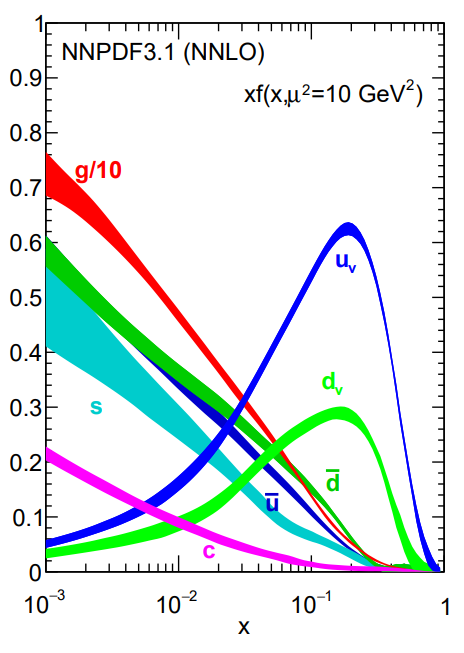
\includegraphics[width=0.7\linewidth]{NNPDF10.PNG}
\end{minipage}
\hfill
\begin{minipage}[t]{0.48\linewidth}
\centering
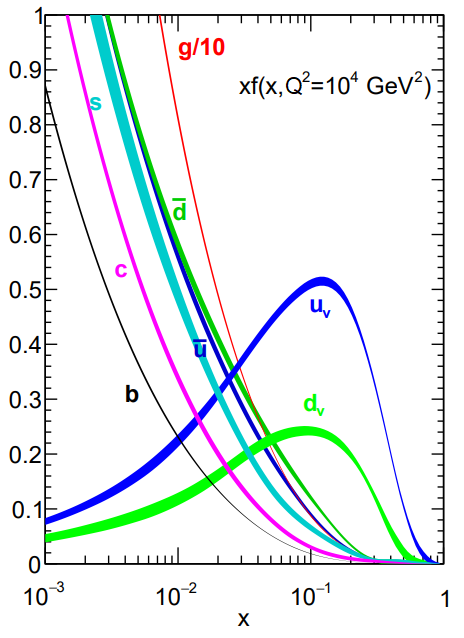
\includegraphics[width=0.7\linewidth]{NNPDF10000.PNG}
\end{minipage}
\vspace{-0.3cm}
\captionof{figure}{ \label{fig:PDFs}
NNPDF partonų pasiskirstymo funkcijų pavyzdžiai \cite{NNPDF}. Kairėje pusėje matomos protono partonų pasiskirstymo funkcijos, kai kvadratinė energija $\mu^{2}=10 \; \mathrm{GeV}^{2}$ o dešinėje -- kai $\mu^{2}=10000 \; \mathrm{GeV}^{2}$. Ant abscisių ašių vaizduojama partono turima protono impulso dalis $x$, o ant ordinačių ašių -- tikimybės tankio vertė $f(x,\; \mu)$, padauginta iš $x$.
}
\end{centering}

\subsubsection{Drell-Yan procesas}
Drell-Yan procesas - tai toks įvykis, kai hadronų susidūrimo metu kvarkas iš vieno hadrono ir antikvarkas iš kito anihiliuoja sukurdami leptono ir antileptono porą. Didžiajame hadronų greitintuve šis procesas vyksta apsikeičiant $Z$ bozonu arba virtualiu fotonu per s-kanalą. Tai galima užrašyti kaip $q\bar{q} \! \rightarrow \! Z/ \gamma^{*} \! \rightarrow \! l^{+}l^{-}$ arba trumpiau $\mathrm{DY} \! \rightarrow \! l^{+}l^{-}$. Drell-Yan proceso Feinmano diagramos pateiktos \ref{fig:dyproc} pav. Teorinis šio proceso tikėtinumas perturbacinėje kvantinėje chromodinamikoje skaičiuojamas antros eilės tikslumu. Eksperimentinis Drell-Yan proceso diferencialinio sklaidos skerspjūvio matavimas teoretikams suteikia galimybes tikslinti ne tik partonų pasiskirstymo funkcijas, bet ir protonų susidūrimo proceso aprašymą (angl.\ \textit{undelying  event}), hadronizacijos modelius, bei teoriškai numatomas aukštesnių eilių pataisas (perturbacinės kvantinės chromodinamikos, elektrosilpnosios sąveikos teorijos) \cite{DY13TeV}. Tam labai svarbu yra kaip įmanoma didesnis eksperimentinių rezultatų tikslumas. Šio darbo metu studijuota Drell-Yan proceso galutinė būsena yra elektrono-pozitrono pora (elektronų kanalas -- $\mathrm{DY} \! \rightarrow \! e^{+}e^{-}$).

\begin{figure}[H]
\centering
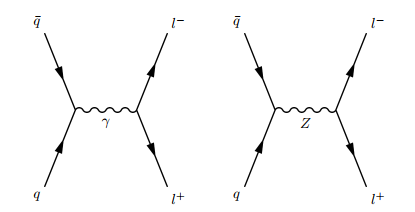
\includegraphics[scale=0.75]{DYprocess.PNG}
\caption{Drell-Yan proceso Feynman'o diagramos.}
\label{fig:dyproc}
\end{figure}

Vienas iš pagrindinių dydžių, matuojamų Drell-Yan proceso tyrime yra diferencialinis sklaidos skerspjūvis $d\sigma/dm$ (čia $m$ -- leptonų (šiuo atveju elektrono-pozitrono) poros \textbf{invariantinė masė}). Brėžiamas diferencialinio sklaidos skerspjūvio grafikas kartais yra vadinamas invariantinės masės spektru. Pagrindinė šio spektro charakteristika yra ta, kad jis yra rezonansinė kreivė -- turi ryškų maksimumą ties $91.2$ GeV ($Z$ bozono masė) ir ties $0$ GeV (fotono masė). Leptonų poros invariantinės masės spektro pavyzdys (kai protonų susidūrimo energija lygi $8$ GeV) pateikiamas \ref{fig:DYeeCS} pav.

Drell-Yan proceso tyrinėjimas taip pat suteikia galimybę ieškoti fizikos už Standartinio modelio ribų, pavyzdžiui, jeigu būtų pastebėtas dar vienas $d\sigma/dm$ maksimumas prie aukštesnių invariantinių masių, būtų galima įtarti $Z'$ bozono egzistavimą ir pan.
\vspace{0.2cm}

\begin{centering}
\begin{figure}[H]
\centering
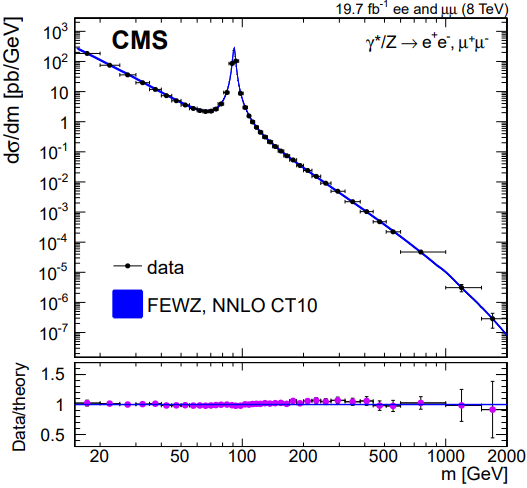
\includegraphics[scale=0.6]{DYeeCS.PNG}
\vspace{-0.2cm}
\caption{\label{fig:DYeeCS}
Drell-Yan proceso invariantinės masės spektras, kai protonų susidūrimo energija lygi $8$ GeV. Mėlyna ištisinė linija žymi teorinį įvertį, apskaičiuotą trečios eilės tikslumu, o juodi taškai -- eksperimentinius duomenis \cite{DYpic}.
}
\end{figure}
\end{centering}

\paragraph{Invariantinė masė} -- tai objekto (rimties) masė, kuri nepriklauso nuo atskaitos sistemos.
Reliatyvistinėje mechanikoje bet dalelės pilnutinė energija $E$ su jos impulsu $\vec{p}$ siejasi tokiu sąryšiu:
\begin{equation}
E^{2}=m_{0}^{2}c^{4} + \left| \vec{p} \right|^{2}c^{2} \; \mathrm{,}
\label{eq:relativity}
\end{equation}
čia $m_{0}$ -- dalelės invariantinė (rimties) masė, $c$ -- šviesos greitis. Prilyginus $c=1$, invariantinė masė bet kokioje atskaitos sistemoje gali būti apskaičiuojama taip:
\begin{equation}
m_{0}^{2}=E^{2}-|\vec{p}|^{2} \; .
\label{eq:invm}
\end{equation}
Jeigu dalelių daugiau negu viena, jų sistemos invariantinė masė $m_\mathrm{system}$ apskaičiuojama taip:
\begin{equation}
m_{\mathrm{system}}^{2}=\left(\sum_{n=1}^{N} E_{n}\right)^{2}-\left|\sum_{m=1}^{N} \vec{p}_{m}\right|^{2} \; .
\label{eq:minvm}
\end{equation}
Dviem dalelėms:
\begin{equation}
m_{12}^2=(E_{1}+E_{2})^{2}-|\vec{p_{1}}+\vec{p_{2}}|^{2} \; .
\label{eq:tinvm}
\end{equation}

\subsection{Drell-Yan proceso eksperimentinis tyrimas}

\subsubsection{Signalas ir triukšmas}
Vykstant didelių energijų dalelių susidūrimams susikuria naujos masyvios dalelės, kurios gyvuoja taip trumpai, kad praktiškai iškart skyla į lengvesnes ir stabilesnes daleles. Pavyzdžiui, $Z$ bozono tikėtiniausia gyvavimo trukmė yra maždaug $3\cdot10^{-25}$ s -- net skriedama labai artimu šviesai greičiu dalelė per tiek laiko nespėtų pajudėti nei per atomo branduolio skersmenį. Kadangi kai kurios dalelės skyla taip greitai ir nespėja praktiškai išvis pajudėti nuo pradinės dalelių susidūrimo vietos, neįmanoma sukurti dalelių detektoriaus, kuris gebėtų detektuoti tokias daleles tiesiogiai. Visi šiuolaikiniai dalelių detektoriai registruoja tik po skilimų ir hadronizacijos susidariusias stabilias daleles, arba čiurkšlėmis vadinamus hadronų (susidariusių kvarkų ir gliuonų hadronizacijos proceso metu) ir kitų stabilių dalelių srautus -- taip vadinamą dalelių susidūrimo įvykio galutinę būseną (angl.\ \textit{final state}).

Kadangi yra daug įvairių dalelių sklaidos procesų, kurių galutinės būsenos sutampa, negalima vienareikšmiškai teikti, kad detektoriaus užfiksuotas įvykis yra būtent tas, kuris mus domina (pavyzdžiui, Drell-Yan proceso įvykis). Taip pat yra galimybė, kad net ir galutinės būsenos dalelė bus atpažinta neteisingai. Taigi eksperimentinėje dalelių fizikoje yra labai svarbu atskirti, kas yra signalas, o kas -- triukšmas, ir įvertinti, kaip triukšmai iškraipo rezultatą.

Šiame tyrime signalu yra vadinama elektrono-pozitrono pora, susidariusi Drell-Yan proceso metu. Triukšmo įvykiai yra bet kokie kiti (ne Drell-Yan) įvykiai, kurių galutinė būsena yra tikrų elektronų pora, arba kitokie dalelių rinkiniai, kurie dėl detektoriaus netobulumo gali būti atpažinti kaip elektronų pora. Kai protonų susidūrimo energija lygi $13$ TeV, tikėtiniausi Drell-Yan proceso triukšmo įvykiai yra šie:
\begin{itemize}
\item $t\bar{t}$ -- viršūninio kvarko skilimas į gelminį kvarką, pozitroną ir elektroninį neutriną ir antiviršūninio kvarko skilimas į atitinkamas antidaleles;
\item $tW$ ir $\bar{t}W$ -- viršūninio arba antiviršūninio kvarko skilimas į gelminį kvarką, pozitroną ir elektroninį neutriną (arba jų antidaleles) ir $W$ bozono skilimas į elektroną ir elektroninį antineutriną (arba jų antidaleles);
\item $\WJets$ -- $W$ bozono skilimas į elektroną\footnote{Toliau dalelės ir antidalelės paprastumo sumetimais bus bendrai vadinamos dalelės vardu, jeigu ir taip pakankamai aišku, kuri dalelė tai turėtų būti. Pavyzdžiui, elektronas ir pozitronas kartu bus vadinami elektronais, nes ir taip aišku, kad $W^{+}$ bozonas skils į pozitroną ir elektroninį antineutriną, o $W^{-}$ bozonas -- atvirkščiai.} ir neutriną bei čiurkšlė kuri buvo klaidingai atpažinta kaip elektronas;
\item $W^{+}W^{-}$ -- dviejų $W$ bozonų skilimas į du elektronus ir du neutrinus;
\item $\WZ$ -- dviejų bozonų skilimas į tris krūvį turinčius leptonus (iš kurių du buvo atpažinti kaip elektronai, o vienas liko neaptiktas) ir vieną neutriną;
\item $\ZZ$ -- dviejų $Z$ bozonų skilimai į keturis leptonus, iš kurių du buvo atpažinti kaip elektronai, o kiti du paliko detektorių neaptikti;
\item $\QCD$ -- procesas, kurio metu susidarė bent dvi čiurkšlės, kurios buvo klaidingai atpažintos kaip elektronai;
\item $\gJets$ -- fotonas ir čiurkšlė, kurie abu buvo klaidingai atpažinti kaip elektronas;
\item $\mathrm{DY} \! \rightarrow \! \tau^{+}\tau^{-}$ -- Drell-Yan proceso taonų kanalas, kai abu taonai skyla į elektronus ir neutrinus.
\end{itemize}

\subsubsection{Įvykių skaičiaus įvertinimo metodai}

Didelių energijų fizikos eksperimentų rezultatai priklauso nuo daugybės faktorių, tokių, kaip procesai, vykstantys dalelių susidūrimo metu, detektorių veikimo ypatumai ir pan. Todėl yra būtina kaip įmanoma tiksliau numatyti eksperimento rezultatus pačiam ir tada tikrinti, ar atlikto eksperimento rezultatai sutampa su iškelta hipoteze. Didelių energijų fizikoje matuojami dalelių susidūrimo įvykiai, todėl čia yra svarbūs įvykių skaičiaus įvertinimo metodai, kurie gali būti teoriniai, eksperimentiniai, arba mišrūs, kurie apjungia abi metodikas tiksliausiam rezultatui pasiekti.

\paragraph{Teoriniai įvykių skaičiaus įvertinimo metodai\\}

Norint padaryti teorinį įvykių skaičiaus įvertį, reikia turėti teorinį modelį, kuriuo remiantis galima apskaičiuoti mus dominančio įvykio $x$ tikimybės pasiskirstymą: tikimybės tankį $f(x)$, arba diskretaus įvykio tikimybę $P(x)$, kurie tenkintų sąlygas $\int_{-\infty}^{\infty}f(x)\mathrm{d}x=1$ arba $\sum_{n=1}^{m}P(x_{n})=1$. Tačiau vien to neužtenka. Reikia turėti galimybę daug kartų (geriausia tiek pat, kiek buvo atliktas pats eksperimentas, arba daugiau) atlikti virtualų eksperimentą, kurio rezultatai priklausytų nuo teorinio tikimybės pasiskirstymo ir gauti teorinį eksperimento rezultatų (įvykių skaičiaus) įvertį. Tai yra padaroma atliekant \textit{Monte Carlo} simuliacijas.

\textit{Monte Carlo} simuliacija (MC) -- tai toks įvykių modeliavimo būdas, kai kompiuteris daug kartų su vienoda tikimybe generuoja atsitiktinius skaičius, kurių vertės būna priskiriamos prie galimų eksperimento baigčių taip, kad atitiktų norimą teorinio pasiskirstymo funkciją, pavyzdžiui binominį, Puasono, Gauso pasiskirstymą ir pan.\ (daugiau skirtingų atsitiktinai generuojamų skaičių verčių priskiriama prie labiau tikėtinų teorinių verčių ir atvirkščiai). Taip principe galima numatyti kiek norime daug skirtingų eksperimentų baigčių (įvykių), kurios, įvykių skaičiui augant į begalybę, pradeda vis idealiau atitikti teorinį pasiskirstymą.

Žinoma, tikri didelių energijų fizikos eksperimentai yra gerokai sudėtingesni ir jų teorinis įvertinimas susideda iš daug skirtingų tikimybinių vyksmų modeliavimo. Pavyzdžiui dažniausiai pirma yra sumodeliuojama daugybė skirtingų protonų susidūrimų baigčių (kokios dalelės susidarė, kokia kryptimi ir kokiu greičiu nulėkė ir pan.), o po to šių modeliavimų rezultatai panaudojami kitame etape, kuriame modeliuojama, kaip dalelių detektorius sureaguos į tokį įvykį ir kokius rezultatus matys eksperimentatoriai. Tokios metodikos privalumas yra tas, kad iš teorinių modelių galima gauti rezultatus (duomenų rinkinius), kurie iš pažiūros atrodo visiškai taip pat, kaip ir tikri eksperimentiniai duomenys. Taip eksperimentatoriams yra labai patogu lyginti, ar jų atlikto eksperimento rezultatai atitinka kokį nors teorinį modelį.

\paragraph{Eksperimentiniai įvykių skaičiaus įvertinimo metodai\\}

Turime tikrus įvykius, jų skaičius baigtinis, tad ir tikimybė (ar jos pasiskirstymas) gaunamas eksperimentinis, kuris, jei teorija teisinga, turėtų artėti į teorinį, kai bandymų skaičius auga į begalybę:
\begin{equation}
P(x)=\lim_{N\rightarrow \infty} \frac{N_{x}}{N} \; .
\label{eq:probLim}
\end{equation}
Tačiau taip paprastai įvykių skaičių ar kitus parametrus išmatuoti būtų galima tik tokiu atveju, jei įvykiai matuojami tiesiogiai (kaip kad pavyzdžiui, liniuote matuojame stalą). Deja, didelių energijų fizikos eksperimentuose, kaip ir praktiškai visose šiuolaikinės fizikos šakose, praktiškai niekas nėra matuojama tiesiogiai (pavyzdžiui, pasinaudodami dujiniu detektoriumi išmatuojame ne dalelę, o elektros srovę, kurią tik galbūt sukėlė dujas jonizavusi pralekianti dalelė). Todėl turime konkrečiai žinoti, ką matuojame ir susikurti modelį, pagal kurį nusimatysime, ką maždaug turėtumėme gauti, jei įvyks būtent tai, ko tikimės. Jeigu tai, ką išmatuojame neatitinka susikurto modelio, remiantis logika ieškoma eksperimento arba modelio trūkumų ir jie šalinami. Todėl tyrimo įranga būna išbandoma su ja atliekant eksperimentus, kurių baigtis jau yra iš anksto žinoma (pavyzdžiui, detektoriaus veikimo patikrinimui galima panaudoti kokią etaloninę medžiagą, kuri spinduliuoja tiksliai žinomos rūšies ir energijos spinduliuotę) kad patikrintume, ar įranga tikrai veikia taip, kaip buvo planuota.

\paragraph{Matavimu grįsti įvykių skaičiaus įvertinimo metodai\\}

Matavimu grįsti metodai apjungia teorinius ir eksperimentinius metodus. Jie naudojami įvertinti triukšmo įvykių skaičiui (tada signalo įvykių skaičių galima apskaičiuoti iš išmatuoto rezultato atėmus triukšmo įvertį). Naudojant matavimu grįstus metodus neretai galima triukšmo įvykių skaičių įvertinti tiksliau, nei naudojant tik vieną iš ankstesnių variantų. Kaip jau ko gero buvo galima suprasti, matavimu grįsti metodai apima matavimą, modeliavimą ir matematinį mechanizmą, kuris sukombinuoja matavimo ir modeliavimo rezultatus į vieną bendrą įvertį.

Egzistuoja daug skirtingų matavimu grįstų triukšmo įvykių skaičiaus įvertinimo metodų, bet jie visi remiasi tuo pačiu pagrindiniu principu. Bet kuriam metodui reikia tam tikrais parametrais apibrėžti taip vadinamą kontrolinę sritį (angl.\ \textit{control region}), kurioje dėl pasirinktų parametrų idealiu atveju liktų vien tik triukšmo įvykiai. Tada apskaičiavus triukšmo įvykių skaičių kontrolinėje srityje pasinaudojant tam tikromis matematinėmis operacijomis įvykių skaičius kontrolinėje srityje transformuojamas į triuškmo įvykių skaičių signalo srityje. Populiariausi metodai, naudojami triukšmo įvykių, kuriuose susidarė hadronų čiurkšlės, skaičiaus įvertinimui, yra klaidingo atpažinimo (angl.\ \textit{fake rate} -- FR) ir ABCD metodai. Kai reikia įvertinti skaičių triukšmo įvykių, kurių galutinėje būsenoje gali susidaryti tiek tos pačios, tiek skirtingų rūšių leptonai, taikomas $e\mu$ metodas.

\paragraph{Klaidingo atpažinimo metodas\\}
Idealiu atveju tikimybė, kad mus dominantis objektas (pavyzdžiui, elektronas) bus atpažintas teisingai yra lygi vienetui, o tikimybė, kad koks nors kitas objektas (pavyzdžiui, čiurkšlė) bus atpažintas kaip mus dominantis lygi nuliui:
\begin{equation}
\begin{cases}
P(e|e)=1\\
P(e|\mathrm{Jet})=0
\end{cases} \; .
\label{eq:rfprob}
\end{equation}
Realybėje taip nėra -- ne visi \ltq{tikri} objektai atpažįstami kaip tokie. Tokių įvykių skaičiaus įvertinimui naudojamas klaidingo atpažinimo metodas (\textit{fake rate method}) Apibrėžiama klaidingai atpažinta (angl.\ \textit{fake}) dalelė. Klaidingo atpažinimo tikimybė -- tai tikimybė, kad mūsų nedominantis (triukšmo) objektas bus identifikuotas kaip tiriamasis objektas. Skirtingi objektai turi skirtingas klaidingo atpažinimo tikimybes. Pavyzdžiui:
\begin{equation}
f_{ej}=P(e|\mathrm{Jet}) \; \mathrm{,}
\label{eq:fr}
\end{equation}
čia $f_{ej}$ -- tikimybė, kad čiurkšlė bus atpažinta kaip elektronas.

Trumpai klaidingo atpažinimo metodo taikymą galima aprašyti taip:
\begin{enumerate}
\item Apskaičiuojama klaidingo atpažinimo tikimybė $f$:

Tai gali būti padaroma iš išmatuotų duomenų rinkinio paimant įvykius pagal labai atsakingai parinktus kriterijus. Turi būti kaip įmanoma labiau užtikrinama, kad visi atrinkti įvykiai yra iš vieno konkretaus proceso, kurio teorinės baigtys yra žinomos. Tada matant rezultatus, kurie atitinka atrankos kriterijus, bet matomos galutinės būsenos dalelės yra tokios, kokios negalėtų susidaryti tokio proceso metu, galima teigti, kad kažkuri užfiksuota dalelė buvo klaidingai atpažinta. Pavyzdžiui, tikimybę, kad elektronas bus klaidingai atpažintas kaip fotonas, galima apskaičiuoti iš užfiksuotų $Z$ bozono skilimų. Tokiu atveju reikėtų atrinkti tokius įvykius, kuriuose buvo aptikti du elektronai, kurių invariantinė masė labai artima $Z$ bozono masei -- maždaug $91.2$ GeV (tokių įvykių skaičių pavadinkime $N_{ee}^{Z}$), arba elektronas ir fotonas, kurių invariantinė masė taip pat labai artima $Z$ bozono masei (tokių įvykių skaičių pavadinkime $N_{e\gamma}^{Z}$). Tinkamai parinkus visus atrankos kriterijus galima būtų spręsti, kad beveik visi tokie įvykiai iš tikrųjų buvo $Z$ bozono įvykiai, tik kartais elektronas buvo klaidingai atpažintas kaip fotonas. Tada galima būtų įvertinti klaidingo atpažinimo tikimybę \cite{FakeRateZ}:
\begin{equation}
f(\gamma|e) = \frac{N_{e\gamma}^{Z}}{2\cdot N_{ee}^{Z}} \; \mathrm{,}
\label{eq:frCalc}
\end{equation}
čia vardiklyje yra dvejetas, nes bet kuris iš dviejų elekronų gali būti klaidingai atpažintas kaip fotonas.
\item Apskaičiuota klaidingo atpažinimo tikimybė $f$ pritaikoma išmatuotiems duomenims:

Skirtingoms dalelėms būdingi skirtingi įvairių jas apibūdinančių dydžių pasiskirstymai, todėl galima pakeisti tam tikrus dalelių atrankos kriterijus taip, kad atranką praeitų beveik vien tik tokios dalelės, kurios ankstesniu atveju atranką praeidavo tik dėl to, kad buvo klaidingai atpažintos kaip mus dominančios -- sukuriama kontrolinė sritis iš beveik vien triukšmo įvykių. Jeigu tariame, kad iš viso buvo $N$ triukšmo įvykių, tai $fN$ iš jų patenka signalo sritį (nes $f$ -- tikimybė, kad objektas bus klaidingai atpažintas, t.y., pateks į signalo sritį), o $(1-f)N$ -- į kontrolinę sritį. Išmatavus triukšmo įvykių skaičių kontrolinėje srityje galima apskaičiuoti įvykių skaičių signalo srytyje:
\begin{equation}
\begin{cases}
N_{\mathrm{BkgSignal}}=fN\\
N_{\mathrm{BkgControl}}=(1-f)N
\end{cases} \; .
\label{eq:bkgsc}
\end{equation}
Išraiškas padaliname vieną iš kitos:
\begin{equation}
\frac{N_{\mathrm{BkgSignal}}}{N_{\mathrm{BkgControl}}}=\frac{f}{1-f} \; .
\label{eq:frBkg}
\end{equation}
Matome, kad pasinaudodami šia formule jau galime transformuoti įvykių skaičių iš kontrolinės srities į triukšmo įvykių skaičių signalo srityje.
\end{enumerate}

\vspace{-0.25cm}
\paragraph{$e\mu$ metodas\\}

$e\mu$ metodas skirtas įvertinti skaičių tokių triukšmo įvykių, kuriuose susidaro dvi nestabilios dalelės, kurios skyla nepriklausomai. Abiems nestabilioms dalelėms turi galioti sąlyga, kad jų skilimo produktuose turi būti vienas elektinį krūvį turintis leptonas. Jeigu tokia sąlyga tenkinama, reiškia yra galimi nestabilių dalelių poros nepriklausomi skilimai į skirtingus leptonus, pavyzdžiui: $t\bar{t}\rightarrow e^{+}e^{-}$, $t\bar{t}\rightarrow\mu^{+}\mu^{-}$, $t\bar{t}\rightarrow\mu^{+}e^{-}$, $t\bar{t}\rightarrow e^{+}\mu^{-}$ (čia kiti nestabilių dalelių skilimo produktai nepažymėti, nes taikant $e\mu$ metodą mums rūpi tik tai, kokie leptonai atsiranda skilimo metu). Atlikus Monte Carlo modeliavimą galima nustatyti teorinį $ee$ (tokie įvykiai, kurių galutinėje būsenoje yra du elekronai) ir $e\mu$ (tokie įvykiai, kurių galutinėje būsenoje yra po vieną elektroną ir miuoną) įvykių skaičiaus santykį, pavyzdžiui: $N_{t\bar{t}}^{ee}/N_{t\bar{t}}^{e\mu}$. Pirmos eilės virsmams šis santykis būtų maždaug 1:2, nes kiekvienai masyviai nestabiliai dalelei tikimybės skilti į elektroną ir miuoną yra praktiškai lygios (ir galime aiškiai matyti, kad iš keturių galimų virsmų du duoda $e\mu$, o tik vienas $ee$). Jeigu tariame, kad $N_{t\bar{t}}^{ee}/N_{t\bar{t}}^{e\mu}=const$, tai galime tikėtis, kad ši konstanta bus tokia pati tiek MC simuliacijoje, tiek eksperimente (idealiu atveju):
\begin{equation}
\frac{N_{t\bar{t}}^{ee , \; \mathrm{Data}}}{N_{t\bar{t}}^{e\mu , \; \mathrm{Data}}}=\frac{N_{t\bar{t}}^{ee , \; \mathrm{MC}}}{N_{t\bar{t}}^{e\mu , \; \mathrm{MC}}} \; .
\label{eq:emuDataMC}
\end{equation}
Aiškiai matome, kad padauginę abi lygties puses iš $N_{t\bar{t}}^{e\mu , \; \mathrm{Data}}$, galime įvertinti, koks turėtų būti $N_{t\bar{t}}^{ee , \; \mathrm{Data}}$:
\begin{equation}
N_{t\bar{t}}^{ee , \; \mathrm{Data}}=\frac{N_{t\bar{t}}^{ee , \; \mathrm{MC}}}{N_{t\bar{t}}^{e\mu , \; \mathrm{MC}}}\cdot N_{t\bar{t}}^{e\mu , \; \mathrm{Data}} \; \mathrm{,}
\label{eq:emuDataMCfix0}
\end{equation}
tik kadangi taip skaičiuojant $N_{t\bar{t}}^{ee , \; \mathrm{Data}}$ jau iš tikrųjų yra įvykių skaičiaus įvertis, būtų teisingiau jį užrašyti kaip $N_{t\bar{t}}^{ee , \; \mathrm{Įvert.}}$:
\begin{equation}
N_{t\bar{t}}^{ee , \; \mathrm{Įvert.}}=\frac{N_{t\bar{t}}^{ee , \; \mathrm{MC}}}{N_{t\bar{t}}^{e\mu , \; \mathrm{MC}}}\cdot N_{t\bar{t}}^{e\mu , \; \mathrm{Data}} \; .
\label{eq:emuDataMCfix}
\end{equation}

Kalbant apie šį metodą kaip apie matavimu grįstą įvykių skaičiaus įvertinimo metodą, sakome, kad įvykiai su $e\mu$ galutine būsena yra kontrolinė sritis. Pavyzdžiui, Drell-Yan proceso metu susidaro elektronų pora, todėl $e\mu$ galutinės būsenos įvykių rinkinyje bus vien tik Drell-Yan proceso triukšmo įvykiai. Taigi $e\mu$ įvykiai šiuo atveju gerai atitinka kontrolinės srities apibrėžimą. Kaip jau ko gero aišku, signalo sritis šiuo atveju yra $ee$ įvykiai, o tada \eqref{eq:emuDataMCfix} formulė yra matematinė operacija, kuria triukšmo įvykių skaičius, apskaičiuotas kontrolinėje srityje, transformuojamas į triukšmo įvykių skaičių signalo srityje.

\subsubsection{Reakcijos skerspjūvis ir integruotas šviesis}

Didelių energijų fizikoje vietoje įprastos bedimensinės tikimybės ir bandymų skaičiaus dažniau yra naudojami tokie fizikiniai dydžiai, kaip reakcijos skerspjūvis ir integruotas šviesis.

Reakcijos skerspjūvis -- tai ploto matavimo vienetus turintis dydis, apibūdinantis tam tikro įvykio tikėtinumą. Šis dydis nėra priklausomas nuo dalelių spindulio intensyvumo ir sufokusavimo, todėl apskaičiuotus reakcijų skerspjūvius galima tiesiogiai lyginti tarp skirtingų dalelių greitintuvų. Išsamesniuose tyrimuose dažnai skaičiuojami diferencialiniai reakcijos skerspjūviai $\mathrm{d}\sigma/\mathrm{d}x$ -- pasiskirstymai, apibrėžiantys reakcijos skerspjūvio priklausomybę nuo tam tikro įvykį aprašančio parametro. Įprastuose sklaidos eksperimentuose dažniausiai skaičiuojamas diferencialinis sklaidos skerspjūvis $\mathrm{d}\sigma/\mathrm{d}\Omega$ -- tikėtinumas, kad dalelė bus išsklaidyta į tam tikrą sferinio kampo dalį $\mathrm{d}\Omega$. Didelių energijų fizikos tyrimuose dažniausiai skaičiuojami kitokie diferencialiniai skerspjūviai -- pavyzdžiui Drell-Yan proceso tyrime skaičiuojamas $\mathrm{d}\sigma/\mathrm{d}m$ -- tikėtinumas, kad įvyks Drell-Yan proceso įvykis, kurio galutinės būsenos elektronų poros invariantinė masė pateks į intervalą $\mathrm{d}m$. Dalelių fizikoje standartintis skerspjūvio matavimo vienetas yra barnas (žymimas $\mathrm{b}$), kuris lygus $10^{-28}\;\mathrm{m}^{2}$.

Šviesis apibrėžiamas kaip dalelių skaičius, pralėkęs pro tam tikrą plotą per laiko vienetą:
\begin{equation}
\mathcal{L}=\frac{1}{\sigma}\frac{\mathrm{d}N}{\mathrm{d}t} \; .
\label{eq:luminosity}
\end{equation}
Suintegravę šviesį per tam tikrą laiką gauname integruotą šviesį: dydį, kuris parodo, kiek dalelių pralėkė tam tikrą plotą per visą eksperimento laiką:
\begin{equation}
\Lumi=\int \mathcal{L}\mathrm{d}t \; .
\label{eq:lumiInt}
\end{equation}
Integruotas šviesis didelių energijų fizikoje dažniausiai matuojamas atvirkštiniais barnais ($\mathrm{b}^{-1}$). Jį galima laikyti savotišku bandymų skaičiumi, kuris turi atvirkštinio ploto dimensiją. Tikėtinas įvykių skaičius $N$, kai žinomas įvykio skerspjūvis $\sigma$ ir integruotas šviesis $\Lumi$, apskaičiuojamas taip:
\begin{equation}
N=\sigma\Lumi \; .
\label{eq:evno}
\end{equation}

\subsubsection{Įvykių modeliavimas}
Didelių energijų dalelių susidūrimams modeliuoti yra yra sukurta daug įvairių programų, kurios skirtos skirtingų procesų modeliavimui, įvykius modeliuoja skirtingu tikslumu (pirmos, antros eilės ir t.t.) ir pan. Nemažiau svarbu yra ir sumodeliuoti, kaip į tam tikrą įvykį sureaguos dalelių detektorius. Detektoriaus atsako modeliavimui taip pat yra sukurta atskiros programinės įrangos, kuri naudoja protonų susidūrimo modeliavimo rezultatus kaip įvestį. Šiame skyrelyje išvardintos šiam darbui aktualiausios modeliavimo programos ir trumpai aprašyta jų paskirtis.
\paragraph{\textsc{Pythia} 8\\}
\textsc{Pythia} 8 -- tai programa, skirta generuoti didelių energijų dalelių susidūrimų Monte Carlo simuliacijoms. Nuo 8.1 versijos \textsc{Pythia} yra parašyta C++ kalba, visos ankstesnės versijos buvo parašytos Fortran kalba. \textsc{Pythia} suteikia kaip įmanoma tikslesnį viso hadronų susidūrimo vaizdą, savyje turi daug teorinių modelių, partonų pasiskirstymo funkcijų. Su \textsc{Pythia} galima modeliuoti tokius dalykus kaip \ltq{kieti} ir \ltq{minkšti} susidūrimai, pradinės ir galutinės būsenų partonų \ltq{dušai}, daugybinės partonų saveikos, protonų spindulio likučiai, fragmentacija (hadronizacija) ir dalelių skilimai \cite{pythia81}. Pythia turi 16 partonų pasiskirstymo funkcijų, į jas įeina ne tik protonų, bet ir tokių dalelių, kaip pionai, pomeronai ir leptonai partonų pasiskirstymo funkcijos. Šį skaičių galima dar išplėsti naudojantis LHAPDF$5$ ir LHAPDF$6$ bibliotekomis.
Su Pythia galima kokybiškai modeliuoti dalelių susidūrimus, kurių energija masių centro sistemoje yra didesnė negu $10$ GeV, ir gali siekti iki $100$ TeV ir daugiau. Įvykiai modeliuojami nulinės eilės (angl.\ \textit{leading order} -- LO) tikslumu \cite{pythia82}.

\paragraph{FEWZ -- \textit{Fully Exclusive W and Z Production}\\}
FEWZ -- tai Fortran pagrindo kodas, skirtas skaičiuoti $W$ ir $Z$ bozonų sukūrimo skerspjūvius hadronų susidūrimuose naudojantis perturbacine kvantine chromodinamika. Jis turi du vykdomuosius failus: FEWZz -- $Z$ procesams ir FEWZw -- $W$ procesams. Į FEWZ taip pat yra įtraukti $W$ ir $Z$ bozonų leptoniniai skilimai su sukinio koreliacijomis, baigtinio pločio efektai, bei $\gamma Z$ interferencija. Į FEWZ yra įtrauktos tokios partonų pasiskirstymo funkcijos, kaip CTEQ, MSTW, ABKM, NNPDF ir kt. FEWZ skaičiuoja įvykius antros eilės perturbacijų tikslumu \cite{fewz}.

\paragraph{GEANT4\\}
C++ kalba parašytos programinės įrangos rinkinys \textsc{Geant4} yra skirtas modeliuoti dalelių sąveiką su medžiaga. \textsc{Geant4} panaudojimo galimybės labai plačios -- galima modeliuoti elektromagnetinius, hadroninius ir optinius procesus, modeliuoti įvykius su daug skirtingų stabilių dalelių, pasirinkti skirtingas medžiagas, kuriomis tos dalelės sklinda ir pan. Įvykius galima modeliuoti labai plačiame energijų diapazone: nuo maždaug $250$ eV iki kelių TeV ir daugiau. Į \textsc{Geant4} siūlomas galimybes taip pat įeina dalelių trekų, pataikymų į detektorių užfiksavimo modeliavimas, skirtingų geometrijų nustatymas ir skirtingų fizikinių modelių pritaikymas \cite{geant4}. \textsc{Geant4} dažniausiai naudojamas viso iš daug komponentų sudaryto dalelių detektoriaus (pavyzdžiui, CMS) atsako modeliavimui, kai jau turimas sumodeliuotas protonų susidūrimo įvykis.

\paragraph{CMSSW -- \textit{CMS SoftWare}\\}
Programinės įrangos rinkinys CMSSW, kurį sudaro CERN CMS detektoriaus duomenų analizės sistema (angl.\ \textit{the framework}), apibrėžianti įvykių duomenų modelį, angl.\ \textit{Event Data Model} -- EDM (bendras CMS eksperimento įvykių duomenų formatas) bei visas kitas paslaugas, reikalingas modeliavimo, kalibravimo, išlygiavimo bei įvykių atkūrimo moduliams, kurie generuoja tokius įvykių duomenis, iš kurių fizikai jau gali daryti duomenų analizę. Pirminis šio karkaso ir visos įrangos tikslas -- palengvinti įvykių atkūrimo ir analizės programinės įrangos plėtojimą ir diegimą \cite{cmsswtwiki}.

CMSSW naudojama ne tik įvykių modeliavimui, bet ir tikrų protonų susidūrimų atkūrimui. Įvykių modeliavimui skirtos programinės įrangos CMSSW yra nemažai (tame tarpe ir \textsc{Pythia}), taip pat yra ir programinė įranga, skirta detektoriaus atsako modeliavimui (pavyzdžiui, \textsc{Geant4})\cite{cmsswev}. 

\subsubsection{Modeliuotų įvykių svorio skaičiavimas}\label{sec:MCweight}

Tarkime, kad tiriame įvykį, kurio skerspjūvis $\sigma$. Tada esant integruotam šviesiui $\Lumi$ turėtų įvykti $N_{0}$ įvykių. Pasinaudojus \eqref{eq:evno} formule, $N_{0}$ apskaičiuojamas taip:
\begin{equation}
\sigma \Lumi=N_{0} \; .
\label{eq:ilumi}
\end{equation}
Kiekvienas realus įvykis turi svorio daugiklį, lygų $1$, tačiau su modeliuotais įvykiais nebūtinai yra taip pat. Susimodeliuoti įvykių galime kiek norime, tik tada reikia jų skaičių sunormuoti į tikrų įvykių skaičių, t.y., kiekvienam modeliuotam įvykiui priskirti po svorio daugiklį. Jeigu turime $N$ sumodeliuotų įvykių, tai kiekvienam iš jų priskyrus po svorio daugiklį ir visus daugiklius susumavus, turėtume gauti jau aptartą įvykių skaičių $N_{0}$:
\begin{equation}
\sum_{i=1}^{N}1\cdot \omega_{i}=N_{0} \; .
\label{eq:wsum}
\end{equation}
Jeigu visi įvykiai buvo sumodeliuoti vienodai, tai gali neštis ir vienodus svorio daugiklius. Tada suma iš \eqref{eq:wsum} supaprastėja į:
\begin{equation}
\sum_{i=1}^{N}1\cdot \omega_{i}=N\omega \; .
\label{eq:swsum}
\end{equation}
Jeigu \eqref{eq:swsum} lygybė galioja, galime sumodeliuoto įvykio svorį apskaičiuoti pagal formulę:
\begin{equation}
\omega=\frac{N_{0}}{N}=\frac{\sigma \Lumi}{N} \; .
\label{eq:weight}
\end{equation}

Kai įvykiai modeliuojami aukštesnių eilių tikslumu, atskirų įvykių svoriai dažniausiai nebesutampa. Tokiu atveju, norint modeliuotų įvykių skaičių sunormuoti į išmatuotų įvykių skaičių, kiekvienam modeliuotam įvykiui  turi būti priskiriamas toks svorinis daugiklis:
\begin{equation}
\omega_{\mathrm{gen}}=\frac{\sigma\Lumi}{\sum_{i=1}^{N}\omega_{i}} \; .
\label{eq:weightnlo}
\end{equation}
Tada pilnutinis kiekvieno įvykio svoris tampa toks:
\begin{equation}
\omega_{i}^{\mathrm{Piln.}}=\omega_{i}\frac{\sigma\Lumi}{\sum_{i=1}^{N}\omega_{i}} \; .
\end{equation}

\subsubsection{Statistinių paklaidų įvertinimas}
Protonų susidūrimo įvykiai, vykstantys Didžiajame hadronų greitintuve yra atsitiktiniai įvykiai, kuriems galioja Puasono pasiskirstymas (sakome \ltq{Puasono įvykiai}). Puasono įvykių skaičiaus paklaida lygi šakniai iš tikėtiniausio įvykių skaičiaus \cite{Poisson}. Kadangi tikėtiniausias įvykių skaičius šiuo atveju nėra žinomas, tai tikrų CMS detektoriumi užfiksuotų įvykių skaičiaus paklaida yra skaičiuojama tiesiog kaip kvadratinė šaknis iš užfiksuotų įvykių skaičiaus:
\begin{equation}
\Delta N^{\mathrm{Data}} = \sqrt{N^{\mathrm{Data}}} \; .
\label{eq:poisUnc}
\end{equation}

Kai įvykių skaičius yra išvestinis dydis (pavyzdžiui, kombinuotas kelių histogramos stulpelių įvykių skaičius, įvykių skaičius, įvertintas $e\mu$ metodu ir pan.), jo paklaida skaičiuojama įprastai:
\begin{equation}
\Delta f(x, y, ...) = \sqrt{\left(\frac{\partial f}{\partial x}\Delta x\right)^{2}+\left(\frac{\partial f}{\partial y}\Delta y\right)^{2}+...} \;\; \mathrm{,}
\label{eq:DerUnc}
\end{equation}

Kadangi modeliuoti įvykiai turi nelygius vienetui svorius, jų skaičiaus paklaida skaičiuojama kaip kvadratinė šaknis iš įvykių svorių kvadratų sumos. Arba, kitaip tariant, jeigu įvykių skaičius yra lygus visų modeliuotų įvykių svorių sumai, tai bendro įvykių skaičiaus paklaida turėtų būti skaičiuojama pagal \eqref{eq:DerUnc} formulę, kurią pritaikius gauname:
\begin{equation}
\Delta N^{\mathrm{MC}} = \sqrt{\sum_{i=1}^{N^{\mathrm{MC}}}w_{i}^{2}} \; .
\label{eq:w2sumUnc}
\end{equation}
Nesunku pamatyti, kad jeigu visų modeliuotų įvykių svoriai būtų lygūs vienetui, \eqref{eq:w2sumUnc} išraiška susilygintų su \eqref{eq:poisUnc}:
\begin{equation}
\Delta N = \sqrt{\sum_{i=1}^{N}1^{2}}=\sqrt{N} \; .
\label{eq:Useless}
\end{equation}

\subsubsection{Sisteminių paklaidų įvertinimas}

Sisteminės įvykių skaičiaus paklaidos pagrinde kyla iš riboto žinojimo, kas tiksliai vyksta protonų susidūrimo metu, koks yra tikrasis Drell-Yan proceso ir triukšmo įvykių skaičius, kaip veikia detektorius, koks tikrasis protonų susidūrimų tankis ir pan. Nors ir tiksliai nežinome, kiek darbo metu gauti įvairūs pasiskirstymai nukrypsta nuo realių pasiskirstymų (nes nežinome, kokie turėtų būti realūs pasiskirstymai), tai vistiek reikia kažkaip kiekybiškai įvertinti. Toliau bus paaiškintas sisteminių paklaidų skaičiavimas elektronų poros invariantinės masės pasiskirstymui. 

Įvairių duomenų analizės parametrų ir manipuliavimo duomenimis būdų pasirinkimas gali turėti įtakos gautam tyrimo rezultatui, todėl jame atsiranda sisteminių nukrypimų. Tarkime, kad vykdydami duomenų analizę galime rinktis tarp dviejų parametrų: $x_{0}$ ir $x_{1}$. Sisteminė paklaida gali būti apibrėžiama kaip skirtumas tarp išmatuoto invariantinės masės pasiskirstymo, kurio vertės priklauso nuo parametro $x$ ir tikrojo invariantinės masės pasiskirstymo $\widetilde{f}(m_{ee})$:
\begin{equation}
\Delta f \left( m_{ee} | x_{i} \right) = \left| \widetilde{f} \left( m_{ee} \right) -
f \left( m_{ee} | x_{i} \right) \right| \, \mathrm{,} \; \; i=0\, , \; 1 \, .
\label{eq:systUncReal}
\end{equation}
Kadangi nežinome, koks turėtų būti tikrasis invariantinės masės pasiskirstymas, tai galime tarti, kad esant skirtingiems parametrams invariantinės masės pasiskirstymo sisteminės paklaidos yra lygiavertės. Tokiu atveju galime invariantinės masės pasiskirstymo sisteminę paklaidą įvertinti kaip skirtumą tarp išmatuotų pasiskirstymų esant skirtingiems parametrams:

\begin{equation}
\Delta f \left( m_{ee} \right) = \left| f \left( m_{ee} | x_{0} \right) - f \left( m_{ee} | x_{1} \right) \right| \; .
\label{eq:SystUncFinal}
\end{equation}

Esant skirtingiems sisteminių nuokrypių šaltiniams bendra sisteminė paklaida skaičiuojama kaip kvadratinė šaknis iš paklaidų kvadratų sumos.

\vspace{-0.3cm}
\subsubsection{Didysis hadronų greitintuvas ir Kompaktiškasis miuonų solenoidas}
Europos branduolinių tyrimų organizacijai CERN priklausantis Didysis hadronų priešpriešinių srautų greitintuvas yra didžiausias ir galingiausias dalelių greitintuvas pasaulyje. Jo žiedo ilgis apie 27 km, ir jis yra maždaug 100 m gylyje po žeme. LHC dažniausiai vykdomi protonų susidūrimai, bet taip pat galimi (ir kartais vykdomi) sunkesnių atomų branduolių susidūrimai. Didžiausia LHC pasiekiama protonų susidūrimų energija siekia $13$ TeV. Protonų susidūrimai jame dažniausiai vyksta kas $25$ ns. Aplink Didįjį hadronų greitintųvą yra išsidėstę septyni dalelių fizikos eksperimentai, didžiausi ir geriausiai žinomi yra du iš jų: CMS ir ATLAS \cite{LHCexperiments}.

Kompaktiškasis miuonų solenoidas (angl.\ \textit{Compact Muon Solenoid} -- CMS) yra plačios paskirties detektorius, galintis aptikti įvairių rūšių daleles, sukurtas protonų (ar kitų dalelių) susidūrimo metu. CMS eksperimente dirbantys mokslininkai užsiima įvairia veikla nuo Standartinio modelio tyrinėjimo iki papildomų dimensijų arba tamsiosios medžiagos paieškų \cite{CMSdetector}.
CMS detektoriaus aukštis ir plotis siekia apie $15$ m, ilgis -- apie $21$ m. Detektoriaus masė siekia maždaug $14000$ tonų, todėl jis yra vadinamas \ltq{kompaktiškuoju} -- kaip toks masyvus jis yra ganėtinai nedidelių matmenų. Detektorius, kaip ir LHC žiedas yra $100$ m po žeme. CMS yra cilindro formos, ant cilindro (angl.\ \textit{barrel}) galų yra uždėti antgaliai (angl.\ \textit{endcaps}) \cite{cmseta}. Jis sudarytas iš daug skirtingų segmentų, skirtų detektuoti skirtingas daleles. Svarbiausia detektoriaus detalė -- superlaidus solenoidas, kuris savo viduje sukuria magnetinį lauką, siekiantį iki $4$ T.

CMS detektoriaus skersinis pjūvis vaizduojamas \ref{fig:CMSslice} pav. Arčiausiai protonų susidūrimo vietos esantis CMS detektoriaus segmentas yra silicio trekų detektorius. Jis susideda iš kelių dalių (pikselinio ir juostinio silicio trekerių), kurios registruoja krūvį turinčių dalelių pradinę lėkio trajektoriją. Aplink silicio trekų detektorių yra išdėstytas elektromagnetinis kalorimetras (angl.\ \textit{electromagnetic calorimeter} -- ECAL). Jis yra pagamintas iš scintiluojančios medžiagos -- švino volframato ($\mathrm{PbWO}_{4}$), į kurią pataikę energingi elektronai arba fotonai sukelia švytėjimą. Švytėjimo intensyvumas proporcingas dalelės energijai, todėl kalorimetre ją galima išmatuoti\cite{Ecal}. Už elektromagnetinio kalorimetro yra sumontuotas hadronų kalorimetras (angl.\ \textit{hadron calorimeter} -- HCAL). Jis pagamintas iš plastiko scintiliatoriaus ir vario sluoksnių. Hadronų kalorimetro paskirtis -- išmatuoti hadronų (dalelių, sudarytų iš kvarkų) energiją. Kalorimetre esančios vario plokštės skirtos prilėtinti lekiančias sunkias daleles. Kadangi energingi hadronai gali prasiskverbti gerokai toliau už elektronus ar fotonus, hadronų kalorimetras yra gerokai storesnis už elektromagnetinį kalorimetrą. Taip pat  dėl šios priežasties dar vienas, plonesnis, hadronų kalorimetro sluoksnis yra sumontuotas už superlaidaus solenoidinio magneto (ta dalis vadinama išoriniu hadronų kalorimetru). Solenoidinio elektromagneto, kurį iš abiejų pusių supa hadronų kalorimetras, paskirtis yra iškreivinti krūvį turinčių dalelių trajektorijas. Iš dalelių trajektorijos kreivumo galima nustatyti jų krūvį bei impulsą. Už išorinio hadronų kalorimetro keliais sluoksniais sumontuoti yra dujiniai miuonų detektoriai. Kadangi miuonai nesąveikauja stipriąja sąveika ir yra pakankamai sunkūs, jie nukeliauja didžiausią atstumą ir todėl jų detektoriai yra toliausiai nuo susidūrimo taško. Miuonai CMS detektoriuje dažniausiai taip ir nesustabdomi, o tik užfiksuojamas jų trekas. Tarp miuonų detektorių yra sumontuotos didžiulės geležies plokštės, kurios apgręžia magnetinį lauką: sustiprina jį netolimoje solenoido išorėje ir neleidžia jam \ltq{išsisklaidyti} toliau nuo detektoriaus. Jos taip pat \ltq{išfiltruoja} daleles, kurios nėra miuonai\cite{Solenoid}.

\begin{figure}[H] \centering
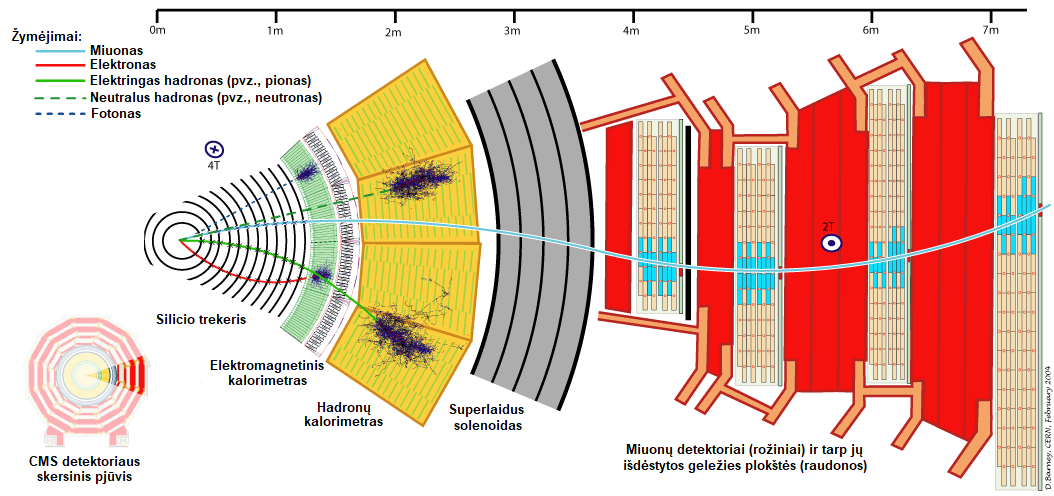
\includegraphics[width=0.95\textwidth]{CMSslice_LT.png}
\vspace{-0.1cm}
\caption{\label{fig:CMSslice}Skersinis CMS detektoriaus pjūvis \cite{CMSslice}. Išorinis hadronų kalorimetras nepavaizduotas. Skirtingų spalvų linijos vaizduoja skirtingų dalelių, sukurtų protonų susidūrimo metu, trajektorijas. Punktyrinė linija reiškia, kad dalelė yra elektriškai neutrali ir nepalieka pėdsako silicio trekų detektoriuje.}
\end{figure}

\paragraph{Sparta ir pseudosparta\\}

Dalelių susidūrimams detektoriuje aprašyti naudojama šiek tiek modifikuota cilindrinė koordinačių sistema. Koordinačių sistemos $z$ ašis nukreipta išilgai protonų spindulių judėjimo krypties ir savo kryptimi sutampa su superlaidaus solenoido kuriamo magnetinio lauko linijų kryptimi. Atstumas nuo koordinačių pradžios taško $r$ ir azimutinis kampas $\phi$ šioje koordinačių sistemoje yra tokie patys kaip ir įprastoje cilindrinėje sistemoje.
Vietoje trečiosios koordinatės dalelių fizikoje dažnai naudojamas dydis, vadinamas sparta. Jis apibrėžiamas taip:
\begin{equation}
y = \frac{1}{2} \ln{ \left( \frac{E+p_{z}c}{E-p_{z}c} \right) } \; \mathrm{,}
\label{eq:rapidity}
\end{equation}
čia $y$ -- sparta, $E$ -- dalelės energija, $p_{z}$ -- dalelės impulso dedamoji išilgai $z$ ašies, $c$ -- šviesos greitis. Spartos kaip koordinatės naudojimo privalumas yra tas, kad dviejų dalelių spartų skirtumas yra invariantas bet kokiose viena kitos atžvilgiu išilgai $Z$ ašies judančiose koordinačių sistemose:
\begin{equation}
y'_{1}-y'_{2}=y_{1}-y_{2}\; \mathrm{,}
\label{rapInvar}
\end{equation}
čia štrichu pažymėtos spartos, apskaičiuotos tariamai judančioje koordinačių sistemoje. Dalelės judėjimo kryptį iš pirminės viršūnės galima pilnai aprašyti žinant spartą $y$ ir azimutinį kampą $\phi$ \cite{pseudorapidity}.

Vis dėlto, šiuolaikiniuose dalelių greitintuvuose sparta taip pat nėra labai patogus dydis, nes jos apskaičiavimui reikia tiksliai žinoti dalelės energijos bei impulso vektoriaus vertes. Tai padaryti, kai dalelės juda reliatyvistiniais greičiais, yra sudėtinga, ypač, kai dalelių sparta yra didelė (dalelės juda beveik išilgai $z$ ašies), nes tada matavimams gali sutrukdyti vamzdis, kuriuo lekia protonų spindulys. Todėl dabar dažniausiai naudojama labai panaši į spartą koordinatė, vadinama pseudosparta. Pseudospartą galima išvesti iš spartos, kai dalelė juda labai artimu šviesai greičiu ir jos rimties energija tampa nepalyginamai mažesnė už kinetinę energiją. Tada pilnutinę dalelės energiją galima apytiksliai užrašyti kaip $E\approx pc$ \cite{pseudorapidity}. Gautas rezultatas -- spartos apiprėžimas -- užrašomas taip:

\begin{equation}
\eta = -\ln \left( \tan \frac{\theta}{2} \right) \; \mathrm{,}
\label{eq:eta}
\end{equation}
čia $\theta$ -- kampas, kurį sudaro dalelės impulso vektorius su $z$ ašimi. Kaip ir sparta, pseudosparta lygi nuliui, kai $\theta=\ang{90}$ ir begalybei, kai $\theta=\ang{0}$. Kampą $\theta$ didinant virš $\ang{90}$ pseudosparta simetriškai mažėja ir pasiekia minus begalybę, kai $\theta=\ang{180}$. Greitintuvuose dalelės judėjimo kryptis iš pirminės viršūnės gali būti pilnai aprašoma pseudospartos ir azimutinio kampo rinkiniu $(\eta, \, \phi)$.

Kadangi detektorius yra išdėstytas aplink protonų spindulį, išmatuoti dalelių energiją išilgai $z$ ašies yra neįmanoma. Dėl šios priežasties matuojami yra tik skersinė energija $E_{\mathrm{T}}$ ir skersinis impulsas $p_{\mathrm{T}}$. Didžiajame hadronų greitintuve sukurtas daleles pilnai aprašantis keturmačio impulso vektorius užrašomas ne kaip $\vec{p}=(p_{x}, \, p_{y}, \, p_{z}, \, E)$ o kaip $\vec{p}=(p_{\mathrm{T}}, \, \eta, \, \phi, \, E)$ arba $\vec{p}=(p_{\mathrm{T}}, \, \eta, \, \phi, \, m)$ (čia prilyginame $c=1$).\\
Skersinis ir pilnutinis dalelės impulsai yra susieti tokia formule:
\begin{equation}
|\vec p|=p_{\mathrm{T}}\cosh\eta \; .
\label{eq:pmodpt}
\end{equation}
Taip pat, kai dalelės aprašomos tokiais keturmačio impulso vektoriais, tai dviejų dalelių invariantinė masė, kuri buvo aprašyta \eqref{eq:tinvm} formulėje, gali būti apskaičiuojama taip:
\begin{equation}
M^2=2p_{\mathrm{T}1}p_{\mathrm{T}2}(\cosh(\eta_{1}-\eta_{2})-\cos(\phi_{1}-\phi_{2})) \; .
\label{eq:ainvm}
\end{equation} 

CMS detektoriaus išilginis pjūvis su kai kurių komponentų pseudospartomis vaizduojamas \ref{fig:cmseta} pav. Tikslesnės detektoriaus komponentų užimamos pseudospartos pateikiamos \ref{table:cmseta} lentelėje.

\begin{table}[H]
\centering
\begin{tabular}{|c|c|}
\hline
CMS komponentas & Pseudosparta $\eta$\\
\hline\hline
Trekeris & $0$ -- $3$\\
\hline
EM kalorimetro cilindras & $0$ -- $1,479$\\
\hline
Hadronų kalorimetro cilindras & $0$ -- $1,4$\\
\hline
Miuonų detektorių cilindras & $0$ -- $1,2$\\
\hline
Superlaidus solenoidas & $0$ -- $1,4$\\
\hline
EM kalorimetro antgalis & $1,479$ -- $3$\\
\hline
Hadronų kalorimetro antgalis & $1,3$ -- $3$\\
\hline
Miuonų detektorių antgalis & $1$ -- $3$\\
\hline
Priekinis hadronų kalorimetras & $3$ -- $5,31$\\
\hline
\end{tabular}
\caption{Apytikslės CMS detektoriaus komponentų pseudospartos (aprašytos tik vienai pusei detektoriaus, prie visų pseudospartų pridėjus minuso ženklą gautume kitos pusės komponentų pseudospartas)\cite{cmseta}.}
\label{table:cmseta}
\end{table}

\begin{figure}[H]
\centering
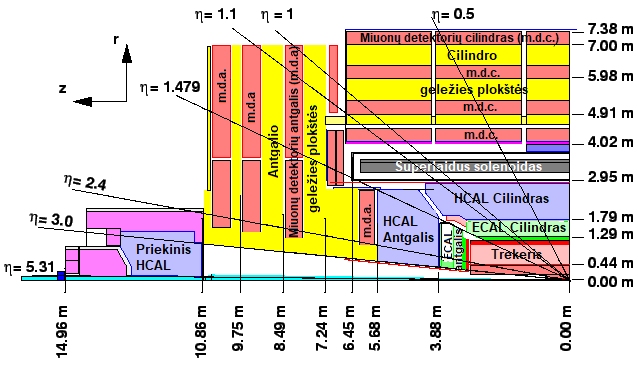
\includegraphics[width=0.85\textwidth]{CMSeta_LT.PNG}
\caption{CMS detektoriaus išilginis pjūvis su pateiktomis kai kurių detektoriaus komponentų pseudospartų vertėmis \cite{cmseta}.}
\label{fig:cmseta}
\end{figure}


\subsubsection{Protonų susidūrimų atkūrimas}\label{sec:ppReco}

Protonams susidūrus susidaro antrinės dalelės (o dažniausiai -- itin trumpai gyvuojančios dalelės), kurias registruojame detektoriumi. Detektoriuose dalelės aptinkamos netiesiogiai. Tai reiškia, kad pralekianti dalelė tik sužadina detektoriuje kokį nors signalą, kurį jau galima išmatuoti, pagal signalo stiprumą kartais galima įvertinti dalelės energiją ir pan. Kad iš to, ką matuoja detektorius, gautume mus iš tikrųjų dominančią informaciją, reikia papildomų skaičiavimų. Norint susidaryti pilną vaizdą, kas įvyko susidūrus protonams, reikia sukombinuoti gautus signalus iš daugybės skirtingų detektoriaus segmentų. Kad galėtume sužinoti, kokios dalelės susidarė, kokia buvo jų energija, kokia trajektorija jos nulėkė, koks dalelių elektrinis krūvis ir pan., reikalinga programinė įranga, kuri tai galėtų daryti daug greičiau ir patikimiau už žmogų. Toliau šiame skyrelyje pateikiamas trumpas paaiškinimas apie dažniausiai naudojamą protonų susidūrimų atkūrimo programinę įrangą.

\paragraph{Dalelių srautas\\}
Dalelių srautas (angl.\ \textit{particle flow}) yra įvykių atkūrimo algoritmas, kuriuo naudjantis protonų susidūrimas atkuriamas pasinaudojant visų CMS detektoriaus komponentų informacija ir atrenkant, kokios galutinės stabilios dalelės susikūrė, bei kuria kryptimi nulėkė. Pradžioje dalelės atrenkamos remiantis labai griežtais atrankos kriterijais ir po sėkmingo atpažinimo atkurti dalelių trekai išimami iš bendro bloko. Tada atrankos kriterijai šiek tiek sušvelninami ir atrankos procesas kartojamas iš naujo (angliškai vadinama \textit{iterative tracking}) -- taip galima efektyviau nustatyti visus dalelių trekus. Vėlesnės iteracijos taip pat nebereikalauja, kad dalelės eitų iš pradinės viršūnės (protonų susidūrimo vietos) -- taip galima nustatyti vėlesnius virsmus, skilimus, spinduliavimą ir pan. Hadronams ir fotonams taikoma gerokai daugiau atrankos kriterijų ir kalibravimo procesų, nei leptonams \cite{pflowpdf}. Po susidūrimo atkūrimo pateikiami duomenys, kurie jau atrodo taip pat, kaip po Monte Carlo įvykio generavimo. Tada Galima iš šio pateikto dalelių sąrašo atkurti ir sudėtingesnius fizikinius objektus, tokius kaip čiurkšlės, trūkstama skersinė energija ir pan.

Taip pat dalelių srautas įvertina kiekvieno atkurto dalelės treko atskirumą (angl.\ \textit{isolation}) -- suskaičiuoja kitų pašalinių dalelių, patekusių į tam tikro pločio kūgį, nubrėžtą aplink tiriamosios dalelės treką, skersinių impulsų sumą \cite{PF2017}. Kuo ši suma mažesnė, tuo trekas atskiresnis. Atskirumo skaičiavimuose taip pat būna įvedamos pataisos, atsižvelgiančios į protonų susidūrimų tankį (keletos skirtingų protonų porų susidūrimai gali įvykti beveik vienu metu ir dalelės, kilusios iš mūsų nedominančių protonų susidūrimų gali trukdyti kokybiškam atskirumo apskaičiavimui) -- įvedamas narys, aprašantis skersinį impulsą dalelių, kurios susidarė ne mus dominančio protonų susidūrimo metu $p_{\mathrm{T}}^{\mathrm{PU}}$. Atskirumą padalinus iš dalelės skersinio impulso, gaunamas santykinis atskirumas. Leptonų santykinis atskirumas skaičiuojamas taip:
\begin{equation}
\label{eq:isolation}
I^{\mathrm{rel.}}_{\mathrm{PF}}= \frac{1}{p_{\mathrm{T}}} 
\left[ \sum_{\Delta R<0.3} p_{\mathrm{T}}^{\mathrm{Ch.\;hadron}}+\mathrm{max}
\left( \sum_{\Delta R<0.3} p_{\mathrm{T}}^{\mathrm{N.\;hadron}}+\sum_{\Delta R<0.3} p_{\mathrm{T}}^{\gamma}-\Delta \beta \sum_{\Delta R<0.3} p_{\mathrm{T}}^{\mathrm{PU}} \, ,\;\; 0 \right) \right] \; \mathrm{,}
\end{equation}
čia $\Delta R = \sqrt{\Delta \phi^{2} + \Delta \eta^{2}} < 0.3$ -- kūgio, brėžiamo aplink leptono trajektoriją, plotis, $\Delta\beta=0.5$ -- iš modeliavimo apskaičiuojamas koeficientas, apytiksliai lygus neutralių ir krūvį turinčių hadronų, susidarančių protonų susidūrimo metu, skaičiaus santykiui.

\paragraph{CMSSW\\}
Naudojantis CMSSW esančiais programinės įrangos paketais galima vykdyti kelių l\~{y}gių įvykio analizę. Iš pradžių vykdoma vietinė detektorių atkūrimas (pataikymai į trekų detektorius, kalorimetrus, miuonų detektoriai), po to jau galima atlikti fizikinių objektų atkūrimas (dalelių trekų nustatymas, atpažinimas, kokios buvo dalelės -- miuonai, fotonai, elektronai, čiurkšlės). Galiausiai atliekama aukšto lygio įvykio atkūrimas (nustatoma trūkstama skersinė energija, kuri reiškia, kad kažkokios dalelės paliko detektorių neaptiktos, nustatoma, ar įvykio metu buvo sukurta tokių sunkių dalelių, kaip taonai ar giluminiai kvarkai, nustatomos viršūnių padėtys ir pan.) \cite{cmsswtwiki}.

\subsubsection{Trigeriai}

Didžiajame hadronų greitintuve protonų susidūrimai dažniausiai vyksta kas $25$ ns. Visų taip dažnai vykstančių susidūrimų išskaityti tiesiog neįmanoma, be to, ir nereikia (kai kurie susidūrimai nepakankamai energingi, kituose galbūt įvyksta tik tie vyksmai, kuriuos laikome jau pakankamai ištirtais ir jie mūsų nedomina ir pan.), todėl yra naudojami trigeriai, kurie sumažina įrašomų įvykių skaičių. Trigeriai būna keleto lygių:
\begin{itemize}
\item Pirmojo lygio (angl.\ \textit{Level-1} -- L1) trigeris

Tai kompiuterių sistema, esanti prie pat detektoriaus. Joje iškart po protonų susikūrimo įvykdomas dalinis įvykio atkūrimas -- apdorojami kalorimetrų ir miuonų detektorių užfiksuoti duomenys. Pagal gautą rezultatą pirmojo lygio trigerio sistema turi \ltq{nuspręsti}, ar įvykis yra vertas dėmesio, ir, jeigu taip, jį įrašyti tolesniam apdorojimui \cite{L1trigger}. Tokiu būdu iš $4\cdot10^{7}$ Hz (įvykių per sekundę) įrašoma tik apie $10^{5}$ Hz \cite{HLtrigger}, o visi kiti įvykiai, kurie neatitinka tam tikrų kriterijų (pavyzdžiui, nėra čiurkšlių, leptonai neatskiri, per maža skersinė energija ir pan.) \ltq{išmetami}. Įvykių atrinkimo kriterijus galima keisti pagal tai, ko ieškoma.
\item Aukšto lygio trigeris (angl.\ \textit{High Level Trigger} -- HLT)

Visi L1 atrinkti įvykiai atsiunčiami į superkompiuterių bloką -- aukšto lygio trigerį -- detalesnei analizei, po kurios įvykių skaičius dar labiau sumažinamas -- maždaug iki $800$ Hz. Čia įvykiai  atkuriami detaliau -- pasinaudojama trekų detektorių užfiksuotais duomenimis, kad būtų atkuriami dalelių trekai, taip pat naudojami sudėtingesni atrankos kriterijai. Trekų atkūrimas sunaudoja daug kompiuterių resursų, todėl pirmojo lygio įvykių atrinkime jis nėra vykdomas \cite{HLtrigger}. Aukšto lygio trigeris atrenka įvykius, kurie su didele tikimybe atitinka konkrečius sklaidos procesus ($W\rightarrow e\nu$, $Z\rightarrow ee$, $H\rightarrow ZZ$ ir pan.), tada jie išskirstomi į grupes pagal panašumą ir įrašomi, kad vėliau galėtų būti tiriami mokslininkų.
\end{itemize}

Šiame darbe buvo naudojami tokie aukšto lygio trigeriai:
\begin{enumerate}
\item Elektrono trigeris, kuris aktyvuojamas, kai aptinkamas bent vienas elektronas, kurio skersinis impulsas yra nemažesnis, nei $23$ GeV. Taip pat šis trigeris netaiko didelių apribojimų elektrono atskirumui.
\item Elektrono ir miuono trigeris, kuris aktyvuojamas, kai užfiksuojamas miuonas, kurio skersinis impulsas $p_{\mathrm{T}}^{\mu}$ yra nemažesnis, nei $8$ GeV ir elektronas, kurio skersinis impulsas $p_{\mathrm{T}}^{e}$ yra nemažesnis, nei $17$ GeV.
\end{enumerate}

\subsubsection{Įvykių atranka}

Protonų susidūrimo įvykių duomenų failai neretai būna plačios paskirties -- įrašyti įvykiai gali būti naudojami skirtingų procesų analizėms. Norint atsirinkti vienai konkrečiai analizei aktualius įvykius, bei kuo užtikrinčiau žinoti, kad duomenyse užregistruotos dalelės yra būtent tos, kurios susidarė iš tikrųjų, yra svarbu pasirinkti tinkamus įvykių atrankos kriterijus, pagal kuriuos yra nusprendžiama, ar įvykis bus naudojamas tolimesnei duomenų analizei. Skirtingiems dalelių rinkiniams yra taikomi skirtingi atrankos kriterijai. Toliau bus aprašomi šiame darbe $ee$ ir $e\mu$ įvykiams taikyti atrankos kriterijai.

\paragraph{$ee$ įvykių atranka\\}
Pirminis atrankos kriterijus elektronų įvykiams buvo ankstesniame skyriuje aprašyto elektrono trigerio suveikimas. Toliau buvo reikalaujama, kad viename įvykyje iš viso būtų aptikti du elektronai, ir kad abu iš jų atitiktų \textit{MediumID} \cite{MediumID8} reikalavimus:

\begin{itemize}
\item Kalorimetro \ltq{dušo} formą apibūdinantis dydis $\sigma_{i\eta i\eta}$ -- elektromagnetinio kalorimetro scintiliuojančių kristalų klasterio plotis išilgai pseudospartos $\eta$, suskaičiuotas visiems $5\!\times\!5$ bloko kristalams (bloko viduryje būtinai yra kristalas, kuriame užfiksuota didžiausia energija);
\item Geometrinis sutapimas tarp superklasterio, į kurį teoriškai pagal atkurtus elektrono parametrus viršūnėje (sukūrimo vietoje) turėjo būti pataikyta, padėties ir išmatuotos superklasterio, į kurį iš tikrųjų buvo pataikyta, padėties: $\Delta \phi_{i\eta}$ ir $\Delta\eta_{i\eta}$;
\item Energijų, paliktų hadronų kalorimetre ir elektromagnetiniame kalorimetre santykis $H/E$;
\item Elektronų atskirumas, apskaičiuotas naudojantis dalelių srauto algoritmu (pagal \eqref{eq:isolation} formulę);

\item Skirtumas tarp atvirkštinės elektrono energijos ir atvirkštinio impulso $1/E-1/P$;
\item Elektrono treko smūgio parametrai statmenoje ir lygiagrečioje plokštumoje, apskaičiuoti atsižvelgiant pirminę viršūnę $|d_{0}|$ ir $|d_{z}|$;
\item Skaičius trekų detektoriaus sluoksnių, kuriuos dalelė praėjo nepalikdama žymių tose vietose, kurios atitinka atkurtą elektrono trajektoriją (trūkstami pataikymai) $N_{e.m.h.}$;
\item Reikalavimas, kad elektronas nebūtų kilęs iš fotono virsmo, apibūdinamas dvejetainiu dydžiu \texttt{PassConversionVeto}.
\end{itemize}
Reikalavimų skaitinės vertės pateiktos \ref{table:eleMediumID} lentelėje.

\begin{table}[H]
\centering
\begin{tabular}{|c|c|c|}
\hline
Kriterijus & Reikalavimai cilindrui & Reikalavimai antgaliams \\
\hline \hline
$\sigma_{i\eta i\eta}$ & $<0.0101$ & $<0.0283$ \\
\hline
$\Delta \phi_{i\eta}$ & $<0.0336$ & $<0.114$ \\
\hline
$\Delta\eta_{i\eta}$ & $<0.0103$ & $<0.00733$ \\
\hline
$H/E$ & $<0.0876$ & $<0.0678$ \\
\hline
$I_{rel}^{PF}$ & $<0.0766$ & $<0.0678$ \\
\hline
$1/E-1/P$ & $<0.0174 \; \mathrm{GeV}^{-1}$ & $<0.0898 \; \mathrm{GeV}^{-1}$ \\
\hline
$|d_{0}|$ & $<0.0118 \; \mathrm{cm}$ & $<0.0739 \; \mathrm{cm}$ \\
\hline
$|d_{z}|$ & $<0.373 \; \mathrm{cm}$ & $<0.602 \; \mathrm{cm}$ \\
\hline
$N_{e.m.h.}$ & $\leqslant 2$ & $\leqslant 1$ \\
\hline
\texttt{PassConversionVeto} & $=$ \texttt{TRUE} & $=$ \texttt{TRUE}\\
\hline
\end{tabular}
\caption{\label{table:eleMediumID}Elektronų atpažinimo \textit{MediumID} reikalavimai $2015$ metų duomenims, kai protonų susidūrimai vyksta kas $25$ ns \cite{MediumID2015}.}
\end{table}
Toliau, kadangi elektromagnetinis kalorimetras efektyviai elektronus detektuoja tik pseudospartos diapazone $|\eta_{SC}| \in [0; 1.4442]\cup[1.566; 2.5)$ ($\eta_{SC}$ -- elektromagnetinio kalorimetro scintiliatorių superklasterio pseudospartos koordinatė), tad ir elektronų kandidatams buvo taikomas reikalavimas patekti į nurodytą pseudospartos diapazoną. Ruožas $1.4442<|\eta_{SC}|<1.566$ \ltq{išmetamas} todėl, kad toje vietoje yra perėjimas iš elektromagnetinio kalorimetro cilindrinės dalies į antgalio dalį. Ten yra išvedžioti laidai, kurie sumažina už jų esančių detektorių efektyvumą. Taip pat neimama pseudosparta, didesnė už $2.5$, nes toje vietoje tiesiog baigiasi elektromagnetinis kalorimetras ir toliau elektronai nedetektuojami.\\
Dar vienas atrankos kriterijus yra elektronų skersinis impulsas: reikalaujama, kad greitesnysis elektronas turėtų skersinį impulsą $p_{\mathrm{T}}^{\mathrm{Gr.}}>30$ GeV, o lėtesnysis -- $p_{\mathrm{T}}^{\mathrm{Lėt.}}>10$ GeV. Nors naudotas elektrono trigeris aktyvuojasi, kai aptinkamas elektronas, kurio $p_{\mathrm{T}}>23$ GeV, jis tai pakankamai efektyviai pradeda daryti tik kai elektronai pasiekia maždaug $p_{\mathrm{T}}^{\mathrm{Gr.}}>30$ GeV impulsą, todėl greitesniajam elektronui (kuris aktyvina trigerį) taikomas būtent toks reikalavimas.
Reikalavimas, kad apskaičiuoti elektronų krūviai būtinai būtų skirtingi, nebuvo taikomas, nes, ypač, kai energijos didesnės, elektronų trajektorijos tampa labai artimos tiesėms, ir efektyvus dalelės krūvio nustatymas yra praktiškai neįmanomas.

\paragraph{$e\mu$ įvykių atranka\\}

Pirminis reikalavimas $e\mu$ įvykiams buvo anksčiau aprašyto elektrono ir miuono trigerio aktyvacija. Taip pat buvo reikalaujama, kad būtų aptikta tik po vieną elektroną ir vieną miuoną. Elektronui toliau buvo taikomi tokie patys atrankos reikalavimai, kaip ir $ee$ įvykių atrankoje, tik dėl naudojamo kitokio trigerio ir kitokio jo veikimo efektyvumo, reikalavimas elektrono skersiniam impulsui buvo pakeistas į $p_{\mathrm{T}}^{e}>25$ GeV.

Miuonas turėjo atitikti \textit{TightID} \cite{TightMuon} reikalavimus:
\begin{itemize}
\item Miuonas turi būti globalus: tai reiškia, kad po įvykio atkūrimo, trekeryje užfiksuotas dalelės, panašios į miuono trekas turi susijungti su miuonų detektoriuose užfiksuotu miuonų treku į vieną bendrą treką;
\item Reikalavimas pagal laisvės laipsnių (angl.\ \textit{degrees of freedom} -- d.o.f.) skaičių normuotam globalaus miuono treko aproksimacijos kokybę apibūdinančiam dydžiui $\chi^{2}/n_{\mathrm{l. \, l.}}<10$;
\item Bent vienas pataikymas į miuonų detektorius turi patekti į aproksimuotą miuono treką;
\item Miuonui turi būti priskirti pataikymai į bent du skirtingus miuonų detektoriaus sluoksnius;
\item Turi būti užkfiksuota bent $6$ miuono pataikymai į skirtingus silicio trekų detektoriaus sluoksnius (iš jų bent vienas į pikselinį detektorių);
\item Reikalavimas treko smūgio parametrui išilginėje statmenoje plokštumoje, apskaičiuotam atsižvelgiant į pirminę viršūnę: $|d_{z}|<0.5$ cm ir $|d_{xy}|<0.2$ cm;
\end{itemize}
Tokie kriterijai gerokai sumažina šansą, kad atranką praeis miuonai, susidarę antrinių procesų metu, taip pat, kad miuonų detektorius pasiekę hadronai, nesustabdyti hadronų kalorimetre, bus klaidingai atpažinti kaip miuonai.

Toliau buvo reikalaujama, kad miuono trekas būtų atskiras: apskaičiuota trekeryje aptiktų dalelių, patenkančių į $\Delta R<0.3$ pločio kūgį, nubrėžtą aplink miuono trajektoriją, impulsų suma neturi viršyti $10\%$ miuono impulso vertės:

\begin{equation*}
\sum_{\Delta R<0.3}p_{\mathrm{T}}<0.1\cdot p_{\mathrm{T}}(\mu) \; .
\end{equation*}

Norint dar efektyviau atskirti, kuriuose įvykiuose miuonai susidarė antrinių procesų metu, arba kitos dalelės buvo klaidingai atpažintos kaip miuonai, galima taikyti reikalavimą ir miuono atskirumui, apskaičiuotam naudojantis dalelių srauto algoritmu (žr. \ref{sec:ppReco} skyrelį).

Kadangi miuonų detektoriai baigiasi ties maždaug $|\eta|=2.4$, tai dar vienu atrankos kriterijumi tapo reikalavimas, kad miuono pseudosparta neviršytų šios vertės: $|\eta_{\mu}|<2.4$. Taip pat dėl trigerio efektyvumo buvo įvestas papildomas apribojimas miuono skersiniam impulsui: $p_{\mathrm{T}}^{\mu}>15$ GeV.

Reikalavimas, kad elektrono ir miuono elektriniai krūviai būtų skirtingi, nebuvo taikomas dėl tos pačios priežasties, kuri buvo paminėta prie $ee$ įvykių atrankos.

\subsubsection{Duomenų analizės biblioteka ROOT}

\vspace{-0.2cm}
Šiame darbe CMS detektoriaus užfiksuotų ir modeliuotų protonų susidūrimų duomenų analizei buvo naudojamas programinės įrangos rinkinys ROOT \cite{ROOT}. ROOT yra galingas įrankis, skirtas didelių duomenų kiekių (angl.\ \textit{Big Data}) apdorojimui, statistinei analizei, vizualizacijai, grafikų braižymui, duomenų saugojimui. ROOT yra parašytas daugiausia C++ kalba, tačiau taip pat yra dalinai integruotas ir su kitomis programavimo kalbomis, tokiomis kaip Python ir R. Duomenų analizei su ROOT buvo rašomi C++ kodai, kurie buvo leidžiami ROOT aplinkoje. ROOT suteikia daug įvairių mokslinei duomenų analizei skirtų klasių bei objektų tipų, todėl C++ kodai, skirti leisti ROOT aplinkoje šiek tiek skiriasi nuo įprastinių C++ kodų. Taip pat, nors ROOT Linux operacinėse sistemose yra paleidžiamas per terminalą, jis vistiek turi šiokią tokią grafinę sąsają, kuria naudojantis galima greičiau peržiūrėti, kas yra saugoma duomenų failuose, šiek tiek paredaguoti išbrėžtus grafikus ir pan.

\paragraph{Protonų susidūrimų duomenys\\}

Visi analizei skirti duomenys buvo saugomi \texttt{.root} formato duomenų failuose. Duomenys šiuose failuose yra sudėti į medžio tipo (\texttt{TTree}) klasę. Medis -- tai tarsi duomenų lentelė. Jame yra skirtingos šakos -- reikšmę turinčiais pavadinimais užkoduotos atminties vietos, kuriose laikomi tam tikro tipo duomenys (pavyzdžiui, detektuotų elektronų skaičius, elektronų energijos ir pan.). Medyje visos šakos kartojasi tiek kartų, kiek įvykių jame įrašoma (kiekvienas įvykis turi tą patį šakų rinkinį, tik jose laiko skirtingas vertes), taigi medį galima įsivaizduoti kaip lentelę, kurios stulpeliai yra šakos (skirtingas reikšmes turintys duomenys), o eilutės -- įvykiai (pirmas užfiksuotas įvykis, antras ir t.t.). Duomenims iš \texttt{.root} failuose esančių medžių nuskaityti reikėjo sukurti klasę, kuri medžius sujungia į grandinę (\texttt{TChain}), iš kurios galima imti medžiuose įrašytus įvykius ir skaityti duomenis, įrašytus šakose. Šią klasę ROOT iš dalies sugeneruoja automatiškai.

\clearpage
\section{Duomenų analizė ir $e\mu$ metodo skaičiavimai}

Šio skyriaus tikslas -- aptarti atlikto darbo metodiką, pažingsniui supažindinti, kas ir kaip buvo daroma, kad būtų pasiektas galutinis šio darbo rezultatas -- Drell-Yan proceso triukšmo įvykių skaičiaus įvertis, apskaičiuotas $e\mu$ metodu, bei suskaičiuotos šio įverčio paklaidos.

\subsection{Modeliuotų duomenų verifikacija}

Visi šiame darbe naudoti duomenys kartu užima apie $200$ GB ir jų visų atrinkimas trunka keletą valandų, todėl klaidų kaina yra nemaža. Norint kuo efektyviau ir tiksliau atlikti eksperimentinių duomenų analizę svarbu yra patikrinti, ar duomenys kokybiškai sumodeliuoti, ar visi įvykių atrankos kodai veikia taip, kaip planuota, ar modeliuotas protonų susidūrimų tankio pasiskirstymas atitinka išmatuotąjį, priskirti modeliuotiems įvykiams teisingus svorius ir pan.

\subsubsection{Modeliuoto Drell-Yan signalo spektro atkūrimas}

Modeliuoto signalo duomenys buvo išskirstyti per keletą duomenų failų (pagal invariantinės masės intervalus, į kuriuos įvykiai patenka). Turint tokius duomenis svarbu yra kiekvieno duomenų failo įvykiams priskirti teisingus svorius, kad tose vietoese, kur baigiasi įvykiai iš vieno failo ir prasideda iš kito, perėjimas būtų tolygus. Šiai užduočiai įvykdyti buvo brėžiamas modeliuoto $\mathrm{DY} \! \rightarrow \! e^{+}e^{-}$ signalo invariantinės masės spektras prieš detektoriaus atsako simuliaciją. Tokio grafiko išbrėžti iš tikrų eksperimentinių duomenų nebūtų galima, nes žinoti, kokie buvo tikrieji dalelių parametrai, galima tik modeliuojant įvykius, o tikruose įvykiuose matoma tik tai, ką išmatavo detektorius. Pirmajam bandymui atkurti sumodeliuotą Drell-Yan signalą buvo naudojami du duomenų failai: viename buvo įrašyti Drell-Yan įvykiai, kurių galutinės būsenos dalelių invariantinė masė yra tarp $10$ ir $50$ GeV, o kitame -- didesnė už $50$ GeV. Gautas Drell-Yan signalo invariantinės masės spektras vaizduojamas \ref{fig:DYMCsignal} pav. Modeliuoti įvykiai turėjo skirtingus individualius svorius, todėl jiems buvo priskiriami svoriai, apskaičiuoti pagal \eqref{eq:weightnlo} formulę. Išbrėžus invariantinės masės histogramą, duomenų iš skirtingų failų susikirtimo vietoje buvo matomas nežymus netolygumas. Histogramų sandūra iš abiejų pusių buvo aproksimuota eksponentinėmis funkcijomis $f(x)=Ae^{-\alpha x}$ (pavaizduota \ref{fig:DYMCfit} pav.). Aproksimacijos kreivių vertės ties $50$ GeV gautos tokios: iš kairės -- $13426.4$, iš dešinės -- $13923.7$, t.y.,  vertės skiriasi apie $3.7\%$, nors turėtų būti apylygės.

Vėliau modeliuoto $\mathrm{DY} \! \rightarrow \! e^{+}e^{-}$ signalo atkūrimui buvo naudojami visi turimi modeliuoto signalo duomenų failai. Kadangi failas su invariantinėmis masėmis, viršijančiomis $50$ GeV, buvo vis dar naudojamas, tik toliau buvo pridėti failai, aprėpiantys $\mathrm{DY} \! \rightarrow \! e^{+}e^{-}$ proceso įvykius su invariantinėmis masėmis nuo $100$ iki $3000$ GeV, pastarojo naudojimui reikėjo įvesti papildomus apribojimus: atmesti įvykius, kurių elektronų poros invariantinė masė patenka į $[100; \, 3000)$ GeV ruožą bei sumažinti šio duomenų rinkinio skerspjūvį iš pradinio rinkinio skerspjūvio atimant visų kitų rinkinių skerspjūvius. Taip buvo gautas šio duomenų rinkinio skerspjūvis, lygus $5790.8$ fb. Toliau įvykių svoriai buvo skaičiuojami pagal anksčiau aprašytą metodiką. Drell-Yan invariantinės masės histograma, gauta naudojant visus modeliuotų duomenų rinkinius, yra pateikiama \ref{fig:DYMCfull} pav.



\vspace{-0.8cm}
\subsubsection{Modeliuotų įvykių peržiūra po detektoriaus atsako modeliavimo}
\vspace{-0.15cm}
Po modeliuoto Drell-Yan signalo patikrinimo buvo bandoma atrinkti modeliuotus įvykius, kuriuose jau sumodeliuotas ir detektoriaus atsakas, ir palyginti juos su eksperimentiniais duomenimis. Prieš atrinkimą modeliuoti duomenys buvo pernormuojami pagal išmatuotą integruotą šviesį: kiekvienam įvykiui buvo priskirtas svoris pagal \eqref{eq:weightnlo} formulę. Vykdant įvykių atranką, elektrono-pozitrono poros ir elektrono-miuono poros susidarymo įvykių atrinkimui buvo naudojami anksčiau aprašyti atrankos kriterijai.

Patikrinimui, ar atrankos koduose nėra klaidų, buvo išbrėžtos elektronų ir miuonų skersinių impulsų ir pseudospartų pasiskirstymų histogramos (\ref{fig:eePtLeadSublead}-\ref{fig:emuEtaMuonEle} pav.). Histogramose aiškiai matosi pritaikyti apribojimai dalelių skersiniams impulsams ir pseudospartoms. Taip pat matyti, kad skersinio impulso histogramos yra tolydžiai gęstančios, pseudospartos pasiskirstymai turi nežymų maksimumą ties $\eta=0$, bei modeliuotų įvykių pasiskirstymai savo forma nuo išmatuotų pasiskirstymų skiriasi labai nežymiai. Tuo remiantis galima spręsti, kad įvykių atranka buvo vykdoma teisingai.

Atliekant $e\mu$ įvykių atranką papildomai buvo tikrinama, ar pasinaudojant dalelių srauto algoritmu apskaičiuoto miuono atskirumo apribojimais galima sumažinti atranką praeinančių $e\mu$ triukšmo įvykių, siejamų su $\WJets$ procesu, skaičių. $\WJets$ procesas yra $e\mu$ triukšmo įvykis, nes greita čiurkšlė gali būti klaidingai atpažįstama kaip atskiras miuonas. Nubrėžta $\WJets$ įvykių atskirumo, apskaičiuojamo naudojantis dalelių srauto algoritmu, histograma (pateiktą \ref{fig:WjetsPFiso} pav.) buvo palyginta su kitų procesų, kuriuose susidaro tikri elektronas ir miuonas, histogramomis (miuono, siejamo su $t\bar{t}$ procesu, atskirumo histograma pateikta \ref{fig:ttbarPFiso} pav.). Buvo pastebėta, kad intervale $I_{\mathrm{PF}}^{\mu}<0.2$ artėjant link nulio $\WJets$ įvykių skaičius stulpelyje auga gerokai lėčiau, nei kitų procesų. Iš to galima spręsti, kad apribojus miuono atskirumą iki $0.1$, galima gan ryškiai sumažinti $e\mu$ atranką praeinančių $\WJets$ įvykių skaičių, tuo pačiu prarandant tik nedidelę dalį įvykių iš visų kitų procesų. Pritaikius šį atrankos kriterijų ir išbrėžus $e\mu$ invariantinės masės histograma buvo įsitikinta, kad taip ir yra.

\subsubsection{Normavimas pagal protonų susidūrimų tankį} \label{sec:PUreweight}
Protonų susidūrimų tankio pasiskirstymai tikruose ir modeliuotuose duomenyse skiriasi ir tai gali turėti įtakos skaičiavimų rezultatams. Šie pasiskirstymai yra vaizduojami \ref{fig:emuNpvMC} pav. Modeliuotus duomenis buvo stengiamasi pernormuoti taip, kad jų pirminių viršūnių skaičiaus pasiskirstymas kuo geriau atitiktų išmatuotąjį. Kiekvienam modeliuotam įvykiui buvo priskirtas svorinis daugiklis pagal tai, kiek pirminių viršūnių buvo atkurta. Kad būtų išvengta dirbtino taškų pritempimo bei atsitiktinių įvykių skaičiaus nukrypimų įtakos, svorinis daugiklis buvo skaičiuojamas išmatuoto ir modeliuoto pirminių viršūnių pasiskirstymų santykį aproksimuojant dvipusio Gauso pasiskirstymu. Taigi, pirmiausia kiekvienas išmatuotų įvykių pirminių viršūnių pasiskirstymo histogramos stulpelis buvo dalinamas iš modeliuotų įvykių pirminių viršūnių pasiskirstymo atitinkamo stulpelio:
\begin{equation}
\label{eq:npvDiv}
F^{\mathrm{\;sant.}}_{0}(N_{\mathrm{PV}})=\frac{F^{\mathrm{Data}}(N_{\mathrm{PV}})}{F^{\mathrm{MC}}(N_{\mathrm{PV}})} \; .
\end{equation}
Kad nebūtų pakeistas normavimas (nepasikeistų sumodeliuotų įvykių skaičiaus), \eqref{eq:npvDiv} formulė dar buvo papildyta pasisiskirstymų integralų santykiu:
\begin{multline}
\label{eq:npvDivNorm}
F^{\mathrm{\;sant.}}(N_{\mathrm{PV}})=
F^{\mathrm{\;sant.}}_{0}(N_{\mathrm{PV}})\cdot
\frac{\int F^{\mathrm{MC}}(N_{\mathrm{PV}}) \mathrm{d}N_{\mathrm{PV}}}
{\int F^{\mathrm{Data}}(N_{\mathrm{PV}}) \mathrm{d}N_{\mathrm{PV}}}=
\\
=\frac{F^{\mathrm{Data}}(N_{\mathrm{PV}})}{F^{\mathrm{MC}}(N_{\mathrm{PV}})}\cdot
\frac{\int F^{\mathrm{MC}}(N_{\mathrm{PV}}) \mathrm{d}N_{\mathrm{PV}}}
{\int F^{\mathrm{Data}}(N_{\mathrm{PV}}) \mathrm{d}N_{\mathrm{PV}}}
\end{multline}

Tada gautas pasiskirstymas $F^{\mathrm{\;sant.}}(N_{\mathrm{PV}})$ buvo aproksimuotas dvipusio Gauso pasiskirstymo funkcija:
\begin{equation}
\bar{F}^{\mathrm{\;sant.}}(N_{\mathrm{PV}})=
\begin{cases} A\cdot \exp\left(-\frac{(x-x_{0})^{2}}{2\sigma_{1}^{2}}\right), & \mbox{kai } x<x_{0} \vspace{0.2cm} \\ 
A\cdot \exp\left(-\frac{(x-x_{0})^{2}}{2\sigma_{2}^{2}}\right), & \mbox{kai } x\geqslant x_{0} \end{cases} \; .
\label{eq:dGauss}
\end{equation}
$F^{\mathrm{\;sant.}}(N_{\mathrm{PV}})$ pasiskirstymai ir jų aproksimacijos vaizduojamos \ref{fig:emuNpvReweight} pav. Aproksimacijos kreivės vertė ties histogramos stulpelio viduriu buvo imama kaip svorio daugiklis modeliuotam įvykiui, kurio pirminių viršūnių skaičius patektų į tą stulpelį. Tas pats buvo daroma tiek su $ee$, tiek su $e\mu$ įvykiais. Gauti galutiniai pirminių viršūnių skaičiaus pasiskirstymai pavaizduoti \ref{fig:emuNpv} pav.

\subsection{$e\mu$ metodo taikymas} \label{sec:emu}
$e\mu$ metodo paskirtis -- patikslinti skaičių tokių įvykių, kurių metu susidaro dvi nestabilios dalelės, kurios nepriklausomai galėjo skilti į bet kurį leptoną su apytiksliai vienoda tikimybe. Šio tyrimo atveju tokie įvykiai būtų $\WW$, $tW$, $\bar{t}W$, $t\bar{t}$, $\DYtau$, tad šis metodas ir buvo taikomas būtent šių procesų (kurių galutinė būsena yra elektronų pora) įvykių skaičiaus patikslinimui. $e\mu$ metodas buvo išbandytas tiek su visais šais procesais kartu, tiek su kiekvienu atskirai, nors \eqref{eq:emuDataMCfix} formulė intuityviausiai būtų tinkama įvertinti visų anksčiau šioje pastraipoje paminėtų procesų įvykių skaičių kartu.

Žvelgiant į šį metodą, kaip į tipinį matavimu grįstą įvykių skaičiaus įvertinimo metodą, galima galvoti, kad tikri CMS detektoriumi išmatuoti $e\mu$ įvykiai yra kontrolinė sritis, o joje apskaičiuotą įvykių skaičių padauginus iš santykio $N^{ee , \; \mathrm{MC}}/N^{e\mu , \; \mathrm{MC}}$ galime transformuoti įvykių skaičių, apkskaičiuotą kontrolinėje srityje į įvykių skaičių signalo srityje. Tačiau žiūrint paprasčiau, šį metodą galime įsivaizduoti kaip modeliuotų $ee$ įvykių skaičiaus pakoregavimą, padauginant jį iš santykio $N^{\mathrm{Data}; \; e\mu}/N^{\mathrm{MC}; \; e\mu}$, kuris idealiu atveju turėtų būti lygus vienetui. Taip galima nesunkiai suprasti, kad dėl to, jog CMS detektoriaus užregistruotų įvykių neįmanoma vienareikšmiškai išskirstyti paprocesiui (matome tik galutinę būseną, o pradinės sužinoti negalime), negalime paprocesiui išskaidyti ir $e\mu$ modeliuotų įvykių (nes kitaip $N^{e\mu, \; \mathrm{Data}}/N^{e\mu , \; \mathrm{MC}}$ nebebus artimas vienetui skaičius). Taigi, taikydami \eqref{eq:emuDataMCfix} formulę kiekvienam procesui atskirai, joje vis tiek imame modeliuotus $e\mu$ įvykius iš visų procesų kartu, o tik modeliuotus $ee$ įvykius imame paprocesiui. Pavyzdžiui, taikant $e\mu$ metodą $\WW$ proceso įvykiams:
\begin{equation}
\label{eq:emuSingleProc}
N_{\WW}^{ee , \; \mathrm{Įvert.}}=N^{e\mu, \; \mathrm{Data}}\cdot\frac{N_{\WW}^{ee , \; \mathrm{MC}}}{N_{\WW}^{e\mu , \; \mathrm{MC}}+N_{tW}^{e\mu , \; \mathrm{MC}}+N_{\bar{t}W}^{e\mu , \; \mathrm{MC}}+N_{t\bar{t}}^{e\mu , \; \mathrm{MC}}+N_{\DYtau}^{e\mu , \; \mathrm{MC}}} \; .
\end{equation}

Tai galima pavadinti vienu iš šio metodo trūkumų -- norint įvertinti kiekvieno triukšmo proceso įvykių skaičių atskirai, modeliuotų įvykių skaičius tikslinamas padauginant jį iš tokio paties daugiklio, kad ir koks tai procesas bebūtų. Tai reiškia, kad neįskaitome to, kad skirtingų procesų modeliavimas gali ne taip pat skirtis nuo realybės. Taigi, domintis vieno konkretaus triukšmo proceso charakteristikomis, šį metodą taikyti būtų ne visiškai tikslinga. Kita vertus, Drell-Yan proceso tyrime mus domina tik kuo tikslesnis bendras visų triukšmo įvykių skaičius (kad galėtume įvertinti, koks įvykių skaičius iš visų užregistruotų $ee$ įvykių buvo būtent Drell-Yan proceso galutinė būsena), tad šiuo atveju aprašytasis $e\mu$ metodo trūkumas jokios įtakos neturi.

Dar vienas šio metodo trūkumas tas, kad jo skaičiavimų tikslumui įtakos turi $e\mu$ įvykių atranką praėję triukšmo įvykiai, tokie, kaip anksčiau aprašyti $\WJets$, taip pat $\gJets$, $\QCD$, bei $\WZ$ ir $\ZZ$. Šie įvykiai mažina $e\mu$ metodo skaičiavimų tikslumą, nes jie nėra tikri $e\mu$ įvykiai. $\WJets$ triukšmai sudaro didžiausią dalį $e\mu$ triukšmo įvykių. Šio įvykio galutinėje būsenoje susidaro vienas tikras leptonas, o čiurkšlė, jeigu yra pakankamai greita, gali būti klaidingai atpažinta, kaip atskiras elektronas arba miuonas. Atranką praėjęs $\gJets$ įvykis reiškia, kad tiek fotonas, tiek čiurkšlė (o $\QCD$ -- kad dvi čiurkšlės) buvo klaidingai atpažinti kaip atskiri leptonai. $\WZ$ ir $\ZZ$ įvykiai $e\mu$ atranką gali praeiti tokiu atveju, kai vienas ($\WZ$ atveju), arba du ($\ZZ$ atveju) leptonai išlekia iš detektoriaus neaptikti. Kadangi $e\mu$ metodas remiasi principu, kad dvi elektringos dalelės nepriklausomai skyla į elektroną arba miuoną su apytiksliai vienoda tikimybe, tai šie procesai $e\mu$ metodo skaičiavimams yra netinkami. Norint kuo tiksliau atlikti skaičiavimus, reikia įvesti korekcijas, kurios į šiuos triukšmus atsižvelgia. Šiame darbe buvo panaudotas paprasčiausias būdas tai įgyvendinti: padaryta prielaida, kad šių triukšmo įvykių ir visų $e\mu$ įvykių santykis yra apytiksliai toks pat tiek matavimui, tiek modeliavimui. Padarę tokią prielaidą galime sumažinti CMS detektoriumi užfiksuotų įvykių skaičių proporcingai pagal triukšmų dalį modeliuotuose $e\mu$ įvykiuose:
\begin{equation}
\label{eq:emu-Wjets_Short}
\widetilde{N}^{e\mu , \; \mathrm{Data}}=N^{e\mu , \; \mathrm{Data}}\cdot\frac{1}{1+R} \; \mathrm{,}
\end{equation}
čia:
\begin{equation}
R=\frac{N_{\WJets}^{e\mu , \; \mathrm{MC}}+N_{\gJets}^{e\mu , \; \mathrm{MC}}+
N_{\WZ}^{e\mu , \; \mathrm{MC}}+N_{\ZZ}^{e\mu , \; \mathrm{MC}}}
{N_{\WW}^{e\mu , \; \mathrm{MC}}+N_{tW}^{e\mu , \; \mathrm{MC}}+N_{\bar{t}W}^{e\mu , \; \mathrm{MC}}+N_{t\bar{t}}^{e\mu , \; \mathrm{MC}}
+N_{\DYtau}^{e\mu , \; \mathrm{MC}}} \; .
\label{eq:emuR}
\end{equation}
Tokia išraiška patogi tuo, kad jeigu triukšmų nėra, $R$ tampa lygus nuliui, o pati trumpena -- vienetui. Bendrai naudotą galutinę $e\mu$ metodo formulę galima užrašyti taip:
\begin{equation}
N_{ee}^{\mathrm{Įvert.}}=\frac{N_{ee}^{\mathrm{MC}}}{N_{e\mu}^{\mathrm{MC}}}\cdot \frac{1}{1+R} \cdot N_{e\mu}^{\mathrm{Data}} \; .
\label{eq:emuLast}
\end{equation}

Kaip bus matyti tolimesniame skyriuje, su $\WJets$ nesusiję $e\mu$ triukšmo įvykiai sudaro gerokai mažesnę dalį $e\mu$ triukmų, nei $\WJets$. Dėl šios priežasties, į \eqref{eq:emuR} išraiškos skaitiklį neįrašę su $\WJets$ nesusijusių įvykių, didelio skirtumo nepastebėsime. Darbe buvo išbandomi $e\mu$ metodo skaičiavimai, kai neįskaitoma nei vieno iš $e\mu$ triukšmo procesų įtaka ($R$ prilyginamas nuliui), kai įskaitoma tik $\WJets$ įtaka, bei kai įskaitomi visi triušmo procesai. Gauti rezultatai bus palyginami kitame skyriuje.

Vis dėlto, šitoks problemos sprendimas nėra idealus todėl, kad pradinė prielaida nebūtinai yra visiškai teisinga. Iš tikrųjų nežinome, ar triukšmo ir visų įvykių santykis tikriems ir modeliuotiems įvykiams yra toks pats. Norint tikslesnių rezultatų, ateityje $\WJets$ ir $\gJets$ įvykiams įvertinti būtų galima naudoti klaidingo atpažinimo metodą.

Taip pat $e\mu$ metodas yra ganėtinai netikslus didelių invariantinių masių ruože, nes ten tikrų $e\mu$ įvykių skaičius yra labai mažas ir atsitiktiniai nukrypimai turi pastebimą įtaką įverčiams -- vienas atranką praėjęs $e\mu$ įvykis gan smarkiai keičia iš \eqref{eq:emuLast} formulės gaunama vertę. Vienas iš šios problemos sprendimo būdų galėtų būti $e\mu$ invariantinės masės pasiskirstymo aproksimavimas tolydžia kreive, tačiau tokiu atveju į skaičiavimus galimai būtų įnešamos papildomos sisteminės paklaidos. Taip pat, Drell-Yan proceso tyrime svarbiausia yra kuo tiksliau žinoti įvykių skaičių $Z$ bozono rezonanso aplinkoje, tad paprastumo dėlei į aprašytą problemą atliekant darbą nebuvo atsižvelgiama. Be to, 2016 ir 2017 metų CMS detektoriaus duomenyse užfiksuotų įvykių yra gerokai daugiau, tad naudojant naujesnius duomenis atsitiktinių nukrypimų įtaka bus mažesnė ir problema dalinai išsispręs savaime.

Pasitikrinimui, ar be klaidų surašytas skaičiavimų kodas, į \ref{eq:emuLast} formulę vietoje tikrų $e\mu$ įvykių buvo paimti modeliuoti $e\mu$ įvykiai, o $R$ prilygintas nuliui. Tokiu atveju metodo įvertis turėtų būti lygus nepakeistam modeliuotų $ee$ įvykių skaičiui.

$e\mu$ metodo skaičiavimai buvo atliekami kiekvienam invariantinės masės histogramos stulpeliui atskirai. Taip pat skaičiavimai buvo išbandyti tiek skaičiuojant kiekvienam procesui atskirai, tiek visiems kartu. \ref{fig:WWest}-\eqref{fig:DYtautauEst} pav.\ vaizduojami $e\mu$ metodo įverčiai, kai skaičiavimai buvo daromi kiekvienam procesui atskirai. Verta atkreipti dėmesį, kad visų procesų $e\mu$ įverčių ir modeliuotų įvykių skaičiaus santykiai atrodo taip pat dėl \eqref{eq:emuSingleProc} formulės specifikos.

\section{Drell-Yan proceso triukšmo įvykių skaičiaus įvertinimo rezultatai}
\vspace{-0.2cm}

Šiame darbe buvo naudojami $ee$ (arba panašios į $ee$) ir $e\mu$ (arba panašios į $e\mu$) galutinių būsenų tikri 2015 metais CMS detektoriaus užfiksuoti protonų susidūrimo įvykiai, bei modeliuoti įvairių procesų įvykiai. Pagrindinis šio darbo tikslas buvo $e\mu$ metodu įvertinti Drell-Yan proceso triukšmo įvykių, siejamų su $\WW$, $tW$, $\bar{t}W$, $t\bar{t}$, $\DYtau$ procesais, skaičių, kad šį rezultatą sukombinavus su modeliavimu būtų galima tikroviškiau įvertinti bendrą $ee$ įvykių skaičių, nei naudojant vien modeliavimą.

\vspace{-0.35cm}
\subsection{Protonų susidūrimų įvykių atrankos rezultatai} \label{sec:ppResults}
\vspace{-0.2cm}

Modeliuotų įvykių normavimo procedūros aprašytos \ref{sec:MCweight} ir \ref{sec:PUreweight} skyriuose. Pagal integruotą šviesį įvykiai buvo pernormuoti priskiriant jiems skerspjūvius, išvardintus \ref{table:CrossSections} lentelėje. Išmatuoti integruoti šviesiai $ee$ ir $e\mu$ duomenų rinkiniuose buvo skirtingi: $2.26$ \invfb  $ee$ įvykiams ir $2.32$ \invfb  $e\mu$ įvykiams. \ref{table:CrossSections} lentelėje taip pat yra pateikiami tikėtini įvykių skaičiai esant $2.26$ \invfb integruotam šviesiui, bei atranką praėjusių modeliuotų dviejų leptonų įvykių skaičiai. Iš viso $ee$ įvykių atranką iš viso praėjo $934135$ tikrų ir $956579$ modeliuotų, o $e\mu$ -- $25817$ tikrų ir $26699$ modeliuotų įvykių, tad modeliavimas pervertina įvykių skaičių. Į su $Z$ bozono rezonansu siejamą invariantinės masės sritį ($60$ -- $120$ GeV) patenka $95.5\%$ tikrų ir $95.8\%$ modeliuotų $ee$ įvykių (labai didele dalimi Drell-Yan įvykiai), bei $44.8\%$ tikrų ir $48.08\%$ modeliuotų $e\mu$ įvykių. 

\vspace{-0.15cm}
\begin{centering}
\begin{table}[H]
\begin{tabular}{|c|c|c|c|c|}
\hline
\multirow{2}{*}{Procesas} & Reakcijos & Tikėtinas įvykių  & Atranką praėjusių & Atranką praėjusių\\
  &  skerspjūvis (pb) & skaičius & $ee$ įvykių skaičius & $e\mu$ įvykių skaičius \\
\hline\hline
$\mathrm{DY} \! \rightarrow \! e^{+}e^{-}$ & $8211.73$ & $1.85585\cdot 10^{7}$ & $939228$ & -- \\
\hline
$\mathrm{DY} \! \rightarrow \! \tau^{+} \tau^{-}$ & $8211.73$ & $1.85585\cdot 10^{7}$ & $2636$ & $5720$ \\
\hline
$t\bar{t}$ & $831.76$ & $1.87978\cdot 10^{6}$ & $7137$ & $17260$ \\
\hline
$\dtW$ & $76.18$ & $1.72167\cdot 10^{5}$ & $800$ & $1792$ \\
\hline
$\WJets$ & $61526$ & $1.39049\cdot 10^{8}$ & $1319$ & $985$ \\
\hline
$\WW$ & $118.7$ & $2.68262\cdot 10^{5}$ & $874$ & $1927$ \\
\hline
$\WZ$ & $47.13$ & $1.06514\cdot 10^{5}$ & $975$ & $187$ \\
\hline
$\ZZ$ & $16.523$ & $3.7432\cdot 10^{4}$ & $675$ & $24$ \\
\hline
$\gJets$ & $3.65896\cdot 10^{5}$ & $8.26925\cdot 10^{8}$ & $86$ & $34$ \\
\hline
$\QCD$ & $5.19096\cdot 10^{6}$ & $1.173157\cdot 10^{10}$ & $2847$ & $490$ \\
\hline
\end{tabular}
\caption{Drell-Yan proceso elektronų kanalo signalas ir pagrindiniai triukšmai, modeliavime naudoti jų reakcijų skerspjūviai, kai protonų susidūrimo energija $\sqrt{s}=13$ TeV, tikėtinas įvykių skaičius, kai protonų susidūrimų integruotas šviesis yra $\Lumi=2.26$~\invfb, bei atranką praėjusių modeliuotų $ee$ ir $e\mu$ įvykių skaičius.}
\label{table:CrossSections}
\end{table}
\end{centering}
\vspace{-0.15cm}

Pasinaudojant dalelių srauto algoritmu apskaičiuojamu miuonų atskirumu buvo sumažintas $e\mu$ įvykių atranką praeinančių $\WJets$ triukšmo įvykių skaičius. Rezultatas atsispindi \ref{fig:emuAfter} paveiksle, kuriame $\WJets$ įvykių skaičius vaizduojamas violetiniuose stulpeliuose. Pritaikius apribojimus atskirumui, apskaičiuojamam naudojantis dalelių srauto algoritmu, šių stulpelių aukštis gerokai sumažėjo.

Gautos modeliuotų ir tikrų $ee$ įvykių invariantinės masės histogramos vaizduojamos \ref{fig:eeInvM} pav., o modeliuotų ir tikrų $e\mu$ įvykių -- \ref{fig:emuInvM} pav.

Pats įvykių atrankos vykdymo procesas užėmė daugiausiai šio darbo laiko. Norint atrinkti visus tikrus ir modeliuotus įvykius su įprastu kompiuteriu užtrunka apie $4$ valandas. Ateityje būtų tikslinga įvairiais būdais pabandyti šį laiką sutrumpinti, pavyzdžiui, efektyvinant kodus, skaičiuojant lygiagrečiai ir pan. Taip pat, atranką galima būtų vykdyti keliais etapais. Pavyzdžiui, vieną kartą įvykių atranką atlikti tik remiantis trigerio aktyvavimu ir užfiksuotų dalelių skaičiumi (ir tokią atranką praėjusius įvykius įrašant į atskirą failą). Tada tolimesnei atrankai, kuriai norime išbandyti įvairesnius kriterijus, naudoti tik pirminę atranką praėjusius įvykius.

%\vspace{-1cm}
\subsubsection{Didelio tikėtinumo įvykiai}
%\vspace{-0.2cm}

\ref{fig:eeInvM}-\ref{fig:emuInvM} pav.\ galima pastebėti, kad kai kurių procesų modeliuotų įvykių skaičiaus pasiskirstymas yra labai netolygus (matosi pavieniai aukšti histogramos stulpeliai). Taip yra todėl, kad tokie įvykiai, kaip $\QCD$ ir $\gJets$ yra labai didelio tikėtinumo (tai matosi \ref{table:CrossSections} lentelėje -- šių procesų tikėtinumas, lyginant su Drell-Yan proceso tikėtinumu, didesnis smarkiau, nei eile). Modeliuojant didelio tikėtinumo įvykius jiems priskiriami labai dideli svoriai. Didelių svorių priskyrimas įvykiams turi savo kainą. Taikant atrankos kriterijus, kurie labai smarkiai sumažina tokių įvykių atrankos praėjimo tikimybę, vistiek atsiranda bent keli įvykiai, kurie sugeba ją praeiti. Tačiau, kadangi tokių įvykių yra labai mažai, o jų svoriai labai dideli, histogramose matome tik keletą aukštų stulpelių. Taip pat, iš \eqref{eq:w2sumUnc} išraiškos matyti, kad didžiausią statistinę paklaidą įneša įvykiai, kurie turi labai didelius svorius. Taigi beveik visą modeliuotų įvykių skaičiaus statistinę paklaidą sudaro $\QCD$ įvykiai (kurie dar ją ir labai išpučia). $\QCD$ įvykių paklaida beveik lygi pačiam įvykių skaičiui (pavyzdžiui, $ee$ atranką praėjo $2847$ įvykiai, o vien $\QCD$ įvykių skaičiaus statistinė paklaida lygi $2797$).

Norint pamatyti realistiškesnį (tolygesnį) tokių įvykių pasiskirstymą bei gauti mažesnes statistines paklaidas, reikėtų turėti labai didelį skaičių įvykių, kad jiems būtų galima priskirti artimus vienetui svorius (pavyzdžiui, šiame darbe naudoti $\QCD$ įvykiai turi svorius, lygius keletui dešimčių ar net šimtų įvykių). Vis dėlto, labai didelis įvykių skaičius nėra patogus laiko ir kompiuterio atminties atžvilgiu, nes bet kuriuo atveju beveik visi tokie įvykiai atrankos metu yra \ltq{išmetami}.

%\vspace{-0.5cm}
\subsection{$e\mu$ metodo rezultatai}
%\vspace{-0.2cm}

\ref{sec:ppResults} skyrelyje buvo paminėta, kad modeliavimas pervertina įvykių skaičių, taigi būtų galima tikėtis, kad, įvertinus įvykių skaičių $e\mu$ metodu, jis turėtų būti sumažintas. Kaip buvo rašoma \ref{sec:emu} skyrelyje, $e\mu$ metodo skaičiavimus buvo bandoma patikslinti įskaitant $\WJets$ ir kitų $e\mu$ triukšmo įvykių įtaką. \ref{table:emu} lentelėje matyti, kad, įvykių skaičius labiausiai sumažinamas, kai įskaitomi visi $e\mu$ triukšmo įvykiai (įvykių skaičiaus sumažėjimas, kai įskaitomi visi triukšmai, ir kai neįskaitomi išvis, skiriasi $2.26$ karto). Vis dėlto, kadangi $\WJets$ yra dominuojantis $e\mu$ triukšmo įvykis, įvykių skaičiaus sumažinimas, kai įskaitoma vien $\WJets$ įtaka, ir kai įskaitomi visi triukšmo procesai, skiriasi tik $15.8\%$. $e\mu$ metodo įverčio, kai atsižvelgiama į visus $e\mu$ triukšmo procesus, palyginimas su modeliavimu pateikiamas \ref{fig:EMuEst} pav. Rezultatas, gaunamas vietoje modeliuotų įvykių įstačius $e\mu$ metodo įverčius, pateikiamas \ref{fig:eeInvMest} pav.
%Matavimo/įverčio santykiai, gauti, kai buvo naudojamas tik modeliuotas įvertis (\ref{fig:eeInvM} pav.), ir kai buvo naudojamas kombinuotas $e\mu$ metodo bei modeliuotas įverčiai (\ref{fig:eeInvMest} pav.), viename grafike yra pavaizduoti \ref{fig:estChange} pav., kad būtų galima pastebėti santykio pasikeitimą dėl $e\mu$ metodo naudojimo.

\begin{centering}
\begin{table}[H]
\begin{tabular}{|c|c|}
\hline
Triukšmų įskaitymas & $e\mu$ metodu įvertintas įvykių skaičius \\
\hline \hline
Triukšmų įtaka neįskaitoma & $4881\pm 64$ \\
\hline
Įskaitomas tik $\WJets$ indėlis & $4715\pm 69$ \\
\hline
Įskaitomi visi $e\mu$ triukšmo procesai & \multirow{2}{5em}{\centering $4668\pm 69$} \\
($\WJets$, $\gJets$, $\QCD$, $\WZ$, $\ZZ$) & \\
\hline
\end{tabular}
\vspace{-0.2cm}
\caption{\label{table:emu} $e\mu$ metodu įvertintas Drell-Yan proceso triukšmo įvykių skaičius su $Z$ bozono rezonansu siejamoje srityje, kai atsižvelgiama į skirtingą $e\mu$ triukšmo procesų skaičių. Nurodytos tik statistinės paklaidos.}
\end{table}
\end{centering}

\begin{centering}
\begin{table}[H]
\begin{tabular}{|c|c|c|c|} %|p{5cm}|p{4cm}|p{8cm}|p{9cm}|
\hline 
\multirow{3}{8em}{\centering Įvykiai} & \multirow{3}{7em}{\centering CMS užfiksuotų įvykių skaičius} & \multirow{3}{9em}{\centering Modeliuotų įvykių skaičius} & \multirow{3}{10em}{\centering Modeliuotų įvykių skaičius taikant $e\mu$ metodo įvertį} \\
 & & & \\
 & & & \\
\hline \hline
\multirow{2}{8em}{\centering $e\mu$} & \multirow{2}{7em}{\centering $25817 \pm 161$} & \multirow{2}{9em}{\centering $26699 \pm 86 \pm 246$ } & \multirow{2}{5em}{\centering \textendash }\\
 & & & \\
\hline
$ee$ ($\WW$, $tW$, $\bar{t}W$, & \multirow{2}{7em}{\centering\textendash} & \multirow{2}{9em}{\centering $11448 \pm 59 \pm 475$} & \multirow{2}{9em}{\centering$\mathbf{10613} \pm 107 \pm 469$} \\
$t\bar{t}$, $\DYtau$) & & & \\
\hline
\multirow{2}{8em}{\centering $ee$ (visi procesai)} & \multirow{2}{7em}{\centering $934135\pm 967$} & \multirow{2}{10em}{\centering $956579\pm 2971\pm11632$} & \multirow{2}{10em}{\centering $\mathbf{955745} \pm 2971 \pm 11656$} \\
 & & & \\
\hline
\multirow{2}{8em}{\centering $N_{ee}/N_{ee}^{\mathrm{Obs.}}$} & \multirow{2}{7em}{\centering 1} & \multirow{2}{10em}{\centering $1.024 \pm 0.003 \pm 0.012$} & \multirow{2}{10em}{\centering $1.023 \pm 0.003 \pm 0.012$} \\
 & & & \\
\hline
\end{tabular}
\caption{\label{table:finalResults} CMS detektoriumi užregistruotų dviejų leptonų įvykių skaičius tirtame dviejų leptonų invariantinės masės intervale. Jeigu prie rezultato pateikiamos dvi paklaidos, tai pirmoji iš jų yra statistinė, o antroji -- sisteminė paklaida.}
\end{table}
\end{centering}

\vspace{-0.3cm}
\begin{centering}
\begin{table}[H]
\begin{tabular}{|c|c|c|c|} %|p{5cm}|p{4cm}|p{8cm}|p{9cm}|
\hline 
\multirow{3}{8em}{\centering Įvykiai} & \multirow{3}{7em}{\centering CMS užfiksuotų įvykių skaičius} & \multirow{3}{9em}{\centering Modeliuotų įvykių skaičius} & \multirow{3}{10em}{\centering Modeliuotų įvykių skaičius taikant $e\mu$ metodo įvertį} \\
 & & & \\
 & & & \\
\hline \hline
\multirow{2}{8em}{\centering $e\mu$} & \multirow{2}{7em}{\centering $11535 \pm 107$} & \multirow{2}{9em}{\centering $12838 \pm 315 \pm 180$ } & \multirow{2}{5em}{\centering \textendash }\\
 & & & \\
\hline
$ee$ ($\WW$, $tW$, $\bar{t}W$, & \multirow{2}{7em}{\centering\textendash} & \multirow{2}{9em}{\centering $5013 \pm 38 \pm 173$} & \multirow{2}{9em}{\centering$\mathbf{4668} \pm 69 \pm 209$} \\
$t\bar{t}$, $\DYtau$) & & & \\
\hline
\multirow{2}{8em}{\centering $ee$ (visi procesai)} & \multirow{2}{7em}{\centering $894660\pm 946$} & \multirow{2}{10em}{\centering $913943 \pm 972 \pm 11201$} & \multirow{2}{10em}{\centering $\mathbf{913598} \pm 973 \pm 11233$} \\
 & & & \\
\hline
\multirow{2}{8em}{\centering $N_{ee}/N_{ee}^{\mathrm{Obs.}}$} & \multirow{2}{7em}{\centering 1} & \multirow{2}{10em}{\centering $1.022 \pm 0.002 \pm 0.013$} & \multirow{2}{10em}{\centering $1.021 \pm 0.002 \pm 0.013$} \\
 & & & \\
\hline
\end{tabular}
\caption{\label{table:finalResultsZ} CMS detektoriumi užregistruotų ir modeliuotų dviejų leptonų įvykių skaičius $Z$ rezonanso aplinkoje ($60$ -- $120$ GeV) Jeigu prie rezultato pateikiamos dvi paklaidos, tai pirmoji iš jų yra statistinė, o antroji -- sisteminė paklaida.}
\end{table}
\end{centering}

%\vspace{-0.3cm}
Nors triukšmo įvykių skaičius invariantinės masės histogramos stulpeliuose iki $700$ GeV yra sumažinamas iki $20\%$, tačiau lyginant įvykių skaičiaus pasikeitimą su visų $ee$ įvykių skaičiumi, šis sieka $0.1\%$. Taip yra todėl, kad bendras visų įvykių skaičius yra labai didelis, o triukšmų skaičius ganėtinai mažas (dominuoja Drell-Yan procesas), todėl bendrame kontekste toks triukšmo įvykių skaičiaus pasikeitimas sunkiai pastebimas, be to, yra nemažas skaičius triukšmo įvykių (išvardinti \ref{table:CrossSections} lentelėje), kurių $e\mu$ metodu įvertinti negalima.
%Į laisvės laipsnių skaičių (invariantinės masės histogramos stulpelių skaičių) normuotas sutapimą tarp matavimo ir (modeliuoto arba $e\mu$ metodo) įverčio apibūdinantis dydis $\chi^{2}/n_{\mathrm{l. \, l.}}$ buvo skaičiuojamas pagal tokią formulę:
%\begin{equation}
%\chi^{2}/n_{\mathrm{l. \, l.}}=\frac{1}{n_{\mathrm{l. \, l.}}} \sum_{i=1}^{n_{\mathrm{l. \, l.}}} \frac{ \left( \rho_{i}^{\mathrm{Įv.}}-\rho_{i}^{\mathrm{Data}} \right) ^{2} }{\rho_{i}^{\mathrm{Data}}} \; \mathrm{,}
%\label{eq:chiSquare}
%\end{equation}
%čia $\rho_{i}^{\mathrm{Įv.}}$ -- modeliuotas ($\rho_{i}^{\mathrm{MC}}$), arba kombinuotas $e\mu$ metodo bei modeliuotas ($\rho_{i}^{\mathrm{MC}+e\mu \, \mathrm{įv.}}$) įvykių skaičiaus tankio įvertis histogramos stulpelyje. Įvykių skaičiaus tankis skaičiuojamas padalinus įvykių skaičių iš stulpelio pločio.
%:
%\begin{equation}
%\rho_{i}=\frac{N_{i}}{m_{\, i \, 1}-m_{\, i \, 0}} \; \mathrm{,}
%\label{eq:numDens}
%\end{equation}
%čia $m_{\, i \, 0}$ ir $m_{\, i \, 1}$ -- $i$-ojo histogramos stulpelio kairysis ir dešinysis rėžiai.
%Iš \eqref{eq:chiSquare} išraiškos matyti, kad kuo $\chi^{2}/n_{\mathrm{l. \, l.}}$ vertė mažesnė, tuo geresnis sutapimas tarp matavimo ir įverčio. Šio dydžio vertės buvo gautos tokios: $\chi^{2}_{\mathrm{MC}}/n_{\mathrm{l. \, l.}}=22.44$; $\chi^{2}_{\mathrm{MC}+e\mu \, \mathrm{įv.}}/n_{\mathrm{l. \, l.}}=22.31$ -- kombinuojant modeliuotą ir $e\mu$ metodo įverčius gaunamas maždaug $0.6\%$ geresnis sutapimas, nei naudojant vien tik modeliavimą.

Gauta $e\mu$ metodo įverčio statistinė paklaida yra $1.82$ karto didesnė už modeliuotų įvykių skaičiaus paklaidą\footnote{Čia nagrinėjami rezultatai, gauti su $Z$ bozono rezonansu siejamoje srityje ($60$ -- $120$ GeV).}. Taip yra todėl, kad įvertis gautas iš kelių duomenų rinkinių, kurių visų statistinės paklaidos įeina į įverčio paklaidą pagal \eqref{eq:DerUnc} formulę. Vis dėlto, statistines paklaidas užgožia apskaičiuotos sisteminės paklaidos. $e\mu$ metodo įverčio sisteminė paklaida už modeliuotų įvykių skaičiaus sisteminę paklaidą yra $21\%$ didesnė. Bendrame kontekste statistinė įverčio paklaida yra maža, lyginant su pilna statistine įvykių skaičiaus paklaida (vien $\QCD$ įvykių skaičiaus statistinė paklaida yra apie $13$ kartų didesnė už $e\mu$ metodo įverčio statistinę paklaidą), taip pat, kaip ir sisteminė paklaida, kuri yra labai maža lyginant su bendra sistemine paklaida, priklausančia nuo trigerių pasirinkimo ir normavimo pagal protonų susidūrimų tankį (bendros sisteminės paklaidos dydis yra lygus $11233$, ji apie $54$ kartus didesnė už $e\mu$ įverčio paklaidą). Taigi bendrame kontekste skirtumas tarp modeliavimo ir $e\mu$ metodo rezultato telpa į paklaidas. Kita vertus, jeigu žiūrime tik į tuos procesus, kurių įvykių skaičių buvo galima įvertinti $e\mu$ metodu, tada modeliavimo ir $e\mu$ įverčio rezultatai yra vienas už kito paklaidų ribų (pačios paklaidos persidengia 52 įvykių intervale), tad galime teigti, kad įvykių skaičiaus įvertintimas $e\mu$ metodu buvo tikslingas.

Tyrimų rezultatai yra apibendrinti \ref{table:finalResults} ir \ref{table:finalResultsZ} lentelėse. Pateikti skaičiai atitinka matavimą detektoriaus geometrinėje erdvėje, kai greitesniojo elektrono $\pT^{\mathrm{Gr.}}>30$ GeV, o lėtesniojo $\pT^{\mathrm{Lėt}}>10$ GeV ($ee$ įvykiams), arba kai elektrono $\pT^{e}>25$ GeV, o miuono $\pT^{\mu}>15$ GeV ($e\mu$ įvykiams).

Norint labiau patikslinti visų procesų įvykių skaičiaus įvertį, reikėtų $e\mu$ metodui netinkamų procesų įvykių skaičių įvertinti kokiu nors kitu matavimu grįstu (pavyzdžiui, klaidingo atpažinimo) metodu, bei patikslinti modeliuotų Drell-Yan signalo įvykių skaičių. Taip pat ateityje sisteminių paklaidų skaičiavime būtų galima pabandyti įtraukti ir daugiau galimų sisteminių nuokrypių šaltinių.

Darbe buvo atsižvelgta į šiuos sisteminių paklaidų šaltinius:
\begin{enumerate}
%\vspace{-0.25cm}
\item Modeliuotų įvykių skaičiaus pokytį dėl pernormavimo pagal protonų susidūrimų tankį;
%\vspace{-0.3cm}
\item Modeliuotų įvykių skaičiaus nesutapimą, kai įvykių atrankai naudojami skirtingi trigeriai;
%\vspace{-0.95cm}
\item Galimai įneštus sisteminius nukrypimus dėl $e\mu$ metodo naudojimo.
\end{enumerate}

%\vspace{-0.15cm}
Parašyti vykdytos duomenų analizės programiniai kodai su minimaliais pataisymais gali būti tinkami naudojimui ir su naujesnių metų CMS detektoriaus duomenimis. Tai buvo išbandyta naudojant šiek tiek skirtingus $2015$ metų duomenų rinkinius.

\clearpage
\section*{Išvados} \addcontentsline{toc}{section}{Išvados}
\begin{enumerate}
\item Didelių energijų fizikos duomenų analizės darbas reikalauja daug laiko ir kruopštumo.
\item Įvertinus Drell-Yan proceso triukšmo įvykių skaičių $e\mu$ metodu, gautas pilnutinis įvykių skaičius buvo artimesnis užregistruotajam CMS detektoriumi, nei naudojant vien tik modeliavimo įvertį ($835$ įvykiais, arba apie $0.1\%$).
\item Vertinant tik tų procesų, kuriems galima taikyti $e\mu$ metodą, įverčius, $e\mu$ ir modeliavimo įverčiai paklaidų ribose nėra tapatūs (modeliavimo įvertis -- $5013\pm38\pm173$, $e\mu$ metodo įvertis -- $4668\pm69\pm209$), tad $e\mu$ metodo taikymas yra tikslingas.
\item $e\mu$ metodo skaičiavimuose atsižvelgus į panašių į $e\mu$ procesų (\ltq{$e\mu$ triukšmų}: $\WJets$ $\gJets$, $\QCD$, $\WZ$, $\ZZ$), kurie iškraipo $e\mu$ įvykių skaičių, egzistavimą, galima pagerinti įvertį.
\item $e\mu$ metodo tikslumas, lyginant su modeliuotu įverčiu, yra žemesnis ($e\mu$ metodu įvertinto įvykių skaičiaus santykinė paklaida -- $4.7\%$, modeliuoto įverčio santykinė paklaida -- $3.6\%$), tačiau gautas įvykių skaičius yra patikimesnis, nes modeliavime yra nežinomų (ir todėl neįskaitomų) neapibrėžtumų.
\item Labai didelio tikėtinumo triukšmo įvykiai su maža tikimybe praeina atrankos kriterijus, todėl jų pasiskirstymą sunku pakankamai tiksliai modeliuoti. Tai nulemia \ltq{pikų} atsiradimą histogramose.
\item Pakeitus miuonų atrankos reikalavimus (vietoje trekerio atskirumo naudojant atskirumą, apskaičiuojamą naudojantis dalelių srauto algoritmu) galima sumažinti $e\mu$ atranką praeinančių $\WJets$ įvykių skaičių.
\item Parašyti protonų susidūrimo įvykių atrankos, $e\mu$ metodo skaičiavimų bei grafikų brėžimo programiniai kodai su minimaliomis korekcijomis galės būti taikomi ir atliekant naujesnių metų CMS duomenų analizę.
\end{enumerate}

\clearpage
%\addtocounter{section}{1}
%\addcontentsline{toc}{section}{\protect\numberline{\thesection}Literatūra}
\addcontentsline{toc}{section}{Literatūros sąrašas}
\bibliography{\jobname}
\bibliographystyle{unsrt}

\clearpage
\section*{Santrauka}
\addcontentsline{toc}{section}{Santrauka (LT)}
\begin{centering}
Marijus Ambrozas\\
\textbf{Drell-Yan proceso triukšmo įvykių skaičiaus įvertinimas $e\mu$ metodu}\\
\end{centering}
\vspace{0.5cm}

Preciziškas Drell-Yan proceso eksperimentinis tyrimas leidžia tikslinti partonų pasiskirstymo funkcijas (angl.\ \textit{parton distribution functions} -- PDF), taip pat įvairius teorinius modelius ir pataisas. Norint gauti kuo tikslesnius Drell-Yan proceso eksperimentinius duomenis, svarbu yra įvertinti Drell-Yan triukšmo įvykių skaičių. Kad būtų sumažinta su matavimu nesusijusių neapibrėžtumų (pvz., nepakankamai tiksliai žinomų įvykių skerspjūvių, detektoriaus atsako modeliavimo netobulumų) įtaka, triukšmo įvykių skaičiaus įvertinimui yra naudojami matavimu grįsti metodai. Šio darbo tikslas buvo $e\mu$ metodu (vienas iš matavimu grįstų metodų) įvertinti $\WW$, $tW$, $\bar{t}W$, $t\bar{t}$ ir $\DYtau$ procesų nulemtų Drell-Yan proceso elektronų kanalo triukšmo įvykių skaičių. Darbe buvo naudojami $2015$ metų CERN CMS detektoriaus duomenys. Kad būtų galima pritaikyti $e\mu$ metodą, visų pirma reikėjo įvykdyti eksperimentinių ir modeliuotų elektrono-pozitrono ($ee$) poros galutinės būsenos bei elektrono ir miuono ($e\mu$) galutinės būsenos įvykių atranką. Modeliuoti įvykiai turėjo būti pernormuoti, kad atitiktų išmatuotąjį integruotą šviesį bei protonų susidūrimų tankį. Tada pasinaudojant $e\mu$ metodu iš CMS detektoriumi registruotų $e\mu$ duomenų, bei modeliuotų $ee$ ir $e\mu$ duomenų buvo apskaičiuotas išvardintų procesų $ee$ galutinės būsenos įvykių skaičiaus įvertis. Vietoje modeliuotų duomenų panaudojus $e\mu$ metodo įvertį gautas rezultatas buvo šiek tiek artimesnis eksperimentiniam rezultatui (minėtų procesų $ee$ galutinės būsenos įvykių skaičius buvo žymiai sumažintas, tačiau, kadangi tai nėra vieninteliai Drell-Yan proceso triukšmai, bendrame kontekste toks sumažėjimas nėra labai aiškiai pastebimas). Taip pat šiame darbe buvo įvertinta įvykių skaičiaus sisteminė paklaida, nulemta trijų skirtingų šaltinių. Darbo metu parašyti programiniai kodai su minimaliomis korekcijomis bus tinkami naudoti su bet kurių metų CMS detektoriaus duomenimis.

\clearpage
\section*{Summary}
\addcontentsline{toc}{section}{Santrauka (EN)}
\begin{centering}
Marijus Ambrozas\\
\textbf{Drell-Yan Process Background Estimation Using $e\mu$ Method}\\
\end{centering}
\vspace{0.5cm}
The precise experimental analysis of the Drell-Yan process allows constraining parton distribution functions (PDFs), as well as testing various theoretical models and corrections. Contribution of background events must be considered in order to perform Drell-Yan measurements as precisely as possible. Some uncertainties in the measurement originate from the simulations of distinct processes, others are related to the response of the detector. These uncertainties can be reduced using data-driven methods. The goal of this work was to estimate the number of Drell-Yan background events originating from $\WW$, $tW$, $\bar{t}W$, $t\bar{t}$ and $\DYtau$ processes using the $e\mu$ method (one of the data-driven methods). The work was performed using CMS detector's data from $2015$. Before using the $e\mu$ method, the electron-positron ($ee$) final state as well as electron-muon ($e\mu$) final state event selection had to be done for the data and MC datasets. The MC events had to be reweighted to match the observed integrated luminosity and the measured distribution of reconstructed vertices. The $e\mu$ method was allowed estimation of the $ee$ final state background events by combining the number of real $e\mu$ data events, MC $e\mu$ events and MC $ee$ events. The final result was obtained by replacing the number of $\WW$, $tW$, $\bar{t}W$, $t\bar{t}$ and $\DYtau$ MC events with the estimated number of Drell-Yan background events. The resultant number of events was a little bit closer to the measured number of events (the number of previously mentioned background events was significantly reduced, but due to the fact that there are more different background processes that could not be estimated using the $e\mu$ method, the reduction of background events did not seem that strong when compared to the full number of events). The systematic uncertainties from three different sources were estimated. The C++ scripts written for this work will be suitable for performing the same analysis with more recent CMS data.

\clearpage
\section*{Bibliografinis aprašas}
%\addcontentsline{toc}{section}{Bibliografinis aprašas}
Marijus Ambrozas. Drell-Yan proceso triukšmo įvykių skaičiaus įvertinimas $e\mu$ metodu. Fizikos bakalauro studijų programos baigiamasis darbas. Vad.\ Andrius Juodagalvis. Vilnius: Vilniaus universitetas, Fizikos fakultetas, 2018.

%\section*{Anotacija}
%\addcontentsline{toc}{section}{Anotacija}
%Eksperimentiniame Drell-Yan proceso tyrime svarbus žingsnis yra triukšmų įvertinimas. Šiame darbe dalis Drell-Yan proceso triukšmo įvykių buvo įvertinta $e\mu$ metodu. Pritaikius šį metodą bendras įvykių skaičiaus įvertis buvo šiek tiek priartintas prie išmatuoto įvykių skaičiaus. Darbe buvo įvertintos skaičiavimų statistinės ir sisteminės paklaidos. Darbas buvo atliekamas rašant programinius kodus ir naudojant 2015 metų CMS detektoriaus duomenis. Parašytus kodus su minimaliomis korekcijomis bus galima naudoti ir su vėlesnių metų CMS detektoriaus duomenimis. 
\end{document}